\RequirePackage{fix-cm}
\documentclass[smallextended]{svjour3}
\usepackage[utf8]{inputenc}
\usepackage{amsmath}%
\usepackage{amsfonts}%
\usepackage{amssymb}%
\usepackage{graphicx}
\usepackage[table, svgnames, dvipsnames]{xcolor}
\usepackage[colorinlistoftodos,
    prependcaption,
    textsize=tiny]{todonotes}
\usepackage{proba}
\usepackage{enumerate}
\usepackage{booktabs}
\usepackage{latexsym}
\usepackage{xargs}
\usepackage{mathptmx}
\usepackage{csquotes}
\usepackage{paralist}
\usepackage[numbers,sort&compress]{natbib}
\usepackage{varioref}
\usepackage[%           % Fine in most cases
            pdfpagelabels,hypertexnames=true,
            plainpages=false,
            naturalnames=false]{hyperref}
\usepackage{color}
\usepackage{booktabs}
\usepackage{siunitx}
\usepackage[section]{placeins}
%\usepackage[symbol]{footmisc}
\definecolor{darkblue}{rgb}{0,0.1,0.5}
\hypersetup{colorlinks,
            linkcolor=darkblue,
            anchorcolor=darkblue,
            citecolor=darkblue}
%
\DeclareMathOperator{\trace}{trace}
%\def\correspondingauthor{\footnote{Corresp%onding author.}}
\newcommandx{\unsure}[2][1=]{%
	\todo[%
        linecolor=gray,
        backgroundcolor=gray!25,
       bordercolor=gray, 
        #1]{#2}
}
\newcommandx{\change}[2][1=]{%
    \todo[
        linecolor=blue,
        backgroundcolor=blue!25,
        bordercolor=blue, #1]{#2}
}
\newcommandx{\info}[2][1=]{%
    \todo[
        linecolor=OliveGreen,
        backgroundcolor=OliveGreen!25,
        bordercolor=OliveGreen, #1]{#2}
}
\newcommandx{\improvement}[2][1=]{
    \todo[linecolor=FireBrick,
        backgroundcolor=FireBrick!25,
        bordercolor=FireBrick,#1]{#2}
}
\newcommandx{\thiswillnotshow}[2][1=]{\todo[disable,#1]{#2}}
\newtheorem{hyp}{Hypothesis}
%-------------------------------------------
\smartqed 
\journalname{Journal of Dynamics and Differential Equations}
\usepackage{scrtime}
% fnpct instead of footmisc:
\usepackage[dont-mess-around]{fnpct}

% patch \maketitle:
\usepackage{etoolbox}
\newcommand*{\affaddr}[1]{#1} % No op here. Customize it for different styles.
\newcommand*{\affmark}[1][*]{\textsuperscript{#1}}
\usepackage{latexsym}
\begin{document}
	\title{%
		Threshold behavior of a stochastic vector plant model.
	}
	\subtitle{%
		The Tomato Yellow Curl Virus
	}
	\author{%
		Gabriel Salcedo-Varela \\ orcid:0000-0002-0147-5089\and 
		Saul Diaz-Infante
	}
	\institute{
		Gabriel Salcedo-Varela \at
		Universidad de Sonora,
		\\
		Departamento de Matem\'aticas, 
		\\
		Boulevard Luis Encinas y Rosales s/n Col. Centro, 
		\\
		Hermosillo, Sonora, CP 83000
		\\
        Tel.: +521 (662)-259-2155, ext. 2394
        \\
        Fax: +521 (662) 259-2219
        \\
        \email{a211203745@unison.mx}
        \and
         Saul Diaz Infante Velasco 
        \at
        CONACYT-Universidad de Soonora,
		\\
		Departamento de Matem\'aticas, 
		\\
		Boulevard Luis Encinas y Rosales
		s/n Col. Centro,		\\
		Hermosillo, Sonora, CP 83000
		\\
        Tel.: +521 (662)-259-2155
        \\
        Fax: +521 (662) 259-2219
        \\
        \email{saul.diazinfante@unison.mx}
	}
	\date{Received: \today / Accepted: date}
	\titlerunning{SDE-vector plant}
	\authorrunning{G. Salcedo-Varela, S. Diaz-Infante}
	\maketitle
	%\keywords{Keywords}
	%
	\begin{abstract}
		BACKGROUND
		\\
		PROBLEM SETUP
		\\
		FINDINGS 
		\\
		IMPLICATIONS
	\end{abstract}
	\
	\section{Introduction}
	    %!TEX root = ../main.tex
\paragraph{Definition of the topic plus background}
\paragraph{Accepted state of the art plus problem to be resolved}
\paragraph{Authors’ objectives}
\paragraph{Introduction to the literature}
%
\paragraph{Survey of pertinent literature}
    [Cite];
    Arwal, Allen, Benito Chen, Holt and Lenhart.
    
\paragraph{Authors’ contribution}
\paragraph{Aim of the present work}
\paragraph{Main results / conclusions}
%
\paragraph{Future implications}
\paragraph{Outline of structure}
	\improvement{Review the structure}
	\section{Deterministic base dynamics}
		\label{sec:model_formulation}
		%!TEX root = ../main.tex
\info{Write deterministic model formulation. Cite Holt. Descrie importatn hypothesis.}
\begin{equation}
	\label{sys::DeterministicSystem} 
	\begin{aligned} 
		\dot{S_p} &= 
			-\beta_p S_p
			\frac{I_v}{N_v} + \tilde{r_1} L_p + \tilde{r_2} I_p  
		\\ 
		\dot{L_p} &= 
			\beta_p S_p
			\frac{I_v}{N_v} - b L_p - \tilde{r_1} L_p  
		\\ 
		\dot{I_p} &= 
			b L_p - \tilde{r_2} I_p  \\ 
		\dot{S_v} &= 
			-\beta_v S_v 
			\frac{I_p}{N_p} - \tilde{\gamma} S_v
			+(1-\theta) \mu  
		\\ 
		\dot{I_v} &= 
			\beta_v S_v \frac{I_p}{N_p} 
			- \tilde{\gamma} I_v
			+ \theta \mu 
			 \\
			S_p(0) &=S_{p0}, 
            L_p(0) = L_{p0},
            I_p(0) = I_{p0},
            \\
             S_v(0) &= S_{v0},
              I_v(0) = I_{v0}
             \\
             N_p(t) &= S_p(t) + L_p(t) + I_p(t),
             \\
             N_v(t) &= S_v(t) + I_v(t),
	\end{aligned} 
\end{equation} 
%\todo{Make a table for description of  all parameters}
\begin{table}
	\begin{center}
		\begin{tabular}{rll} 
			\toprule
			Par. & Unit & Description 
			\\ 
			\midrule
				$\beta_p$ 
				& 
					\SI{}{vector \per day}
				& 
					infection rate of susceptible 
					plants by infected vectors 
			\\ 
				$r_1$, $r_2$ 
				& 
					$\SI{}{day}^{-1}$ 
				& 
					replanting rate of latent and 
					infected plants, respectively. 
			\\
				$b$ 
				& 
					$\SI{}{day}^{-1}$ 
				& 
					latency rate, plant latent 
					becomes infectious 
			\\
				$\gamma$ 
				& 
					$\SI{}{day}^{-1}$ 
				&  vector death rate 
			\\
				$\mu$ 
				& \SI{}{plant \per day}
				& vector migration rates from alternative plants to crop
			\\
				$\theta$ 
				& 
				& proportion vector migration rate
			\\
				$\beta_v$ 
				& \SI{}{plant\per day}
				& infection rate of susceptible vectors by an infected plant
			\\
			\bottomrule
		\end{tabular}
	\end{center}
	\caption{
		Parameters description and values of
		deterministic dynamics in ODE (*).
	}
	\label{tbl:deterministic_tbl}
\end{table}
%\info{Add initial conditions}
%
\begin{table}
	\begin{center}
		\begin{tabular}{rllll} 
			\toprule
			Par. & Deterministic & Extinction by Noise & $R^s_0<1$ & $R^s_0>1$ 
			\\ 
			\midrule
				$\beta_p$ 
				& 
                    0.1
                &
				    0.05 
				& 
				    0.01 
				& 
				    0.8 
			\\ 
				$r_1$
				&
				    0.01
				&
				    0.9 
				& 
				    0.9
				& 
				    0.6
			\\
				$r_2$ 
				&
				    0.01
				&
				    0.005 
				& 
				    0.9 
				& 
				    0.6
			\\
				$b$ 
				&
				    0.075
				&
				    0.9 
				&   
				    0.5
				& 
				    0.5 
			\\
				$\gamma$ 
				&
				    0.06
				&
				    0.3
				& 
				    0.74247636 
				& 
				    0.06
			\\
				$\mu$ 
				&
				    0.3
				&
				    0.3 
				& 
				    0.058596601 
				& 
				0.058596601
			\\
				$\theta$ 
				&
				    0.4
				&
				    0.0 
				&   
				    0.818469652
				&   
				    0.818469652
			\\
				$\beta_v$ 
			    &
			        0.003
			    &
			        0.1 
			    & 
			        0.227718623 
			    & 
			        0.8
			\\
			    $\sigma_p$ 
			    &
			        -
			    &
			        0.3 
			    & 
			        0.378173863 
			    & 
			        0.378173863
			\\
                $\sigma_v$ 
                & 
                    -
                &
                    0.3 
                & 
                    0.254146903 
                & 
                    0.254146903 
            \\
			\bottomrule
		\end{tabular}
	\end{center}
	\caption{
		Parameters values of
		stochastic dynamics.
	}
	\label{tbl:value}
	\end{table}

%\todo{%Redact this conservation law to the entire system \autoref{sys::DeterministicSystem}.
%Write a introductory paragraph to Thm 1}

Note that we have conservation laws for populations of plants and vectors.
In the plant population, we have a constant population conservation law.
Whereas for vector population, we do not have a constant population, but we bound
the total population by a positive constant. \autoref{thm::conservationlaw}
shows the bound for each law conservation.

\begin{theorem}\label{thm::conservationlaw}
	With the notation of ODE \eqref{sys::DeterministicSystem}, let
	\begin{equation*}
		\begin{aligned}
		 	N_v^{\infty} &:= \frac{\mu}{\gamma}.
		 \end{aligned}
	\end{equation*}
	Then for any initial condition 
	$
		(S_p(0), L_p(0), I_p(0), S_v(0), I_v(0) )^\top
	 	\in \Gamma
	$, plant and vector total populations respectively satisfies
	\begin{equation*}
		\begin{aligned}
			& \frac{d N_p}{dt} =
				\frac{d}{dt}(S_p + L_p + I_p) = 0,
			\\
			& \lim_{t\to \infty}
				N_v(t) = N_v^{\infty}.
		\end{aligned}
	\end{equation*}
\end{theorem}

		\subsection{Deterministic fixed points}
			%\change{
			    %Move definition of invariant set to this section.
			  %  Write a paragraph about Positivity invariance
			    %Compute $R_O$ and write paragraphs to
			    %describe fixed points. Fist Free disease.
			%} 
			%!TEX root = ../main.tex
%\todo{Fix notation to distinguish between free disease and endemic}

To see the positivity invariance we have to make all coordinates zero except for
one. In \autoref{sys::DeterministicSystem}it is quickly observed that there is
invariance when $ S_p = L_p = I_p = 0 $, in the case when $ S_v = 0 $ or 
$ I_p = 0 $, the flow of dynamics is always positive. Therefore
\autoref{sys::DeterministicSystem} is positive invariant.

Let $\R^n_+$ the first octant of $\R ^ n$ and consider  
$$	{
	\Gamma:= 
		\left \{ 
			(S_p, L_p, I_p, S_v, I_v)^{\top} \in \R^5_+: \quad
			0\leq S_p + L_p + I_p \leq N_p, \quad
			S_v + I_v \leq \frac{\mu}{\gamma}
		\right \},
	}
$$
Here we compute the deterministic fixed points of system 
\eqref{sys::DeterministicSystem} and show that its unicity. Thus by definition of we solve 
%
\begin{equation}
	\begin{aligned}
		-\beta_p S_p \frac{I_v}{N_v} + r(N_p-S_p) &= 0\\
		\beta_p S_p \frac{I_v}{N_v} - b L_p - r L_p &= 0\\
		b L_p - r I_p &= 0\\
		-\beta_v S_v \frac{I_p}{N_p} -\gamma S_v +(1-\theta) \mu &= 0\\
		\beta_v S_v \frac{I_p}{N_p} -\gamma I_v + \theta \mu &= 0.
	\end{aligned}
\end{equation}
to determine our fixed points.
%
There is two fixed points\textemdash free disease equilibrium and the 
endemic equilibrium. We characterize the fist the relation
$ L^*_p=I_p^*=I_v^*=0$, which implies that
%
\begin{equation*}
	r(N_p-S^*_p) = 0,
\end{equation*}
%
and therefore, we obtain $S_p^*=N_p$.F or the vector population we have by 
\autoref{thm::conservationlaw} that $S_v^*+I_v^* \rightarrow \frac{\mu}{\gamma}$ as 
$\rightarrow \infty$, then $S_v^* \rightarrow \frac{\mu}{\gamma}$ when we have 
$I^*_v=0$.
%
The free disease equilibrium point is $(N_p,0,0,\frac{\mu}{\gamma},0)^{\top}$. 
For the case of endemic equilibrium point, we need suppose that $L_p^{**},I_p^{**},I_
v^{**}\neq0$ and solve each right hand side of system \autoref{sys::DeterministicSystem} in terms
of other variable.
%
From $\dot{S_p}$, we can obtain
%
\begin{equation*}
	S^{**}_p= \frac{rN_{{p}}N_{{v}}}{rN_{{v}}+I^{**}_v\beta_{{p}}},
\end{equation*}
%
 and similar for the other equations we obtain
\begin{equation*}
	\begin{aligned}
		L^{**}_p &= \frac{\beta_{{p}}S_p^{**} I_v^{**}}{N_{{v}} \left( b+r \right)},
		\\
		I^{**}_p &=\frac{b L^{**}_p}{r},
		\\
		S^{**}_v &=
			\frac{
				\left( 
					1-\theta 
				\right) 
				\mu\, N_{p}
			}{
				\gamma\, N_{p} + I^{**}_ p
				\beta_{v}
			},
	\end{aligned}
\end{equation*}
%
Expresing the above coordinate in terms of $I^{**}_v$, we obtain
%
%\improvement{rewrite as align}
%
\begin{equation*}
	\begin{aligned}
	S^{**}_p &= 
		\frac{
			r N_p N_v
		}{
			r N_v + 
			I^{**}_v 
			\beta_p
		},
	\\
	L^{**}_p &= 
		\frac{
			\beta_p rN_p I^{**}_v
		}{
			\left( 
				b + r 
			\right)
			(
				r N_v + I_v^{**} 
				\beta_p
			)
		},
%
%
	\\
	I^{**}_p &=
		\frac{
			b \beta_p N_p I_v^{**}
		}{
			 \left(
			 	 b + r 
			 \right)
			 ( r N_v + 
			 	I_v^{**} \beta_p
			 )
		},
	\\
	S^{**}_v &=
		\frac{
			 \left( 
			 	1 - \theta 
			 \right)
			 \mu(b + r)
			 (rN_v + \beta_p I_v^{**})
		}{
			\gamma(b + r)
			(r N_v + \beta_p I^{**}_v) + 
			b \beta_p \beta_v I_v^{**}
		},
	\end{aligned}
\end{equation*}
%
%
We only need substituting the above expression into the differential equation 
of $I_v$ and solve the following quadratic equation
%
	\begin{multline}
		-N_p [ 
			b \gamma^2 r I^{**}_v N_v +
			b \gamma^2 (I^{**}_v)^2 \beta_p -
			b \gamma \mu r \theta N_v - 
			b \gamma \mu \theta I^{**}_v \beta_p + 
			\\
			b \gamma (I^{**}_v)^2 \beta_p \beta_v + 
			b \mu \theta I^{**}_v \beta_p ^ 2
			-
			b \mu \theta I^{**}_v \beta_p \beta_v +
			\gamma^2 r^2 I^{**}_v N_v +
			\\
			\gamma^2 r (I ^{**}_v) ^ 2 \beta_p - 
			\gamma\mu r^2 \theta N_v - 
			\gamma\mu r \theta I^{**}_v +
			\beta_p - b\mu I^{**}_v \beta_p^2
		] = 0 \ .
	\end{multline}
% 
In sake of clearness we define 
\begin{align*}
	a_1 &:= 
		b \gamma^2 \beta_p + 
		b \gamma \beta_p \beta_v + 
		\gamma^2 r \beta_p
		,\\
	a_2 &:=-b \gamma \mu \theta \beta_p + 
		b \mu \theta \beta_p ^ 2 - 
		b \mu \theta \beta_p \beta_v + 
		\gamma^2 r^2 N_v - 
		\gamma \mu r 
		\theta \beta_p - 
		b \mu \beta_p^ 2 + 
		\gamma ^ 2 r N_v,
	\\
	a_3 &:=-b\gamma\mu r\theta N_v-\gamma\mu r^2\theta N_v, 
\end{align*}
%
and rewrite the above equation in this new notation as

\begin{equation}\label{eqn::QuadraticInfectedFP}
    \begin{aligned}
    	&\underbrace{
    		(
    		b \gamma^2 \beta_p + 
    		b \gamma \beta_p \beta_v + 
    		\gamma^2 r \beta_p
    		)
    	    }_{:=a_1} I_v^{**2}\\
    	&+ 
    	\underbrace{
    	(-b \gamma \mu \theta \beta_p + 
    		b \mu \theta \beta_p ^ 2 - 
    		b \mu \theta \beta_p \beta_v + 
    		\gamma^2 r^2 N_v - 
    		\gamma \mu r 
    		\theta \beta_p - 
    		b \mu \beta_p^ 2 + 
    		\gamma ^ 2 r N_v
    		)
    		}_{:=a_2} I^{**}_v \\
    		&- 
    	\underbrace{
    	(b\gamma\mu r\theta N_v+\gamma\mu r^2\theta N_v
    	)}_{:=a_3}=0 \ .
\end{aligned}
\end{equation}

%\todo{Fill according to each term}
We need a positive solution, then according to discriminant, we obtain
\begin{equation*}
	\begin{aligned}
		\Delta &= 
		a_2  ^ 2 -  4a_1 a_3
		\\
		&=
			(
				- b \gamma \mu \theta \beta_p +
				b \mu \theta \beta_p^2 -
				b \mu \theta \beta_p \beta_v + 
				\gamma ^ 2 r ^ 2 N_v - 
				\gamma \mu r \theta \beta_p - 
				b \mu \beta_p ^ 2 + 
				\gamma ^ 2 r N_v 
			) ^ 2
		\\
		& +  
		%
		4( 
			b \gamma ^ 2 \beta_p + 
			b \gamma \beta_p
			\beta_v + 
			\gamma^2 r \beta_p
		)
		%
		(
			b \gamma \mu r 
			\theta N_v + 
			\gamma \mu r ^ 2 \theta N_v
		),			
	\end{aligned}	
\end{equation*}
which ever is positive, then we have two different real solution, 
since we require the positive, we deduce that
\begin{equation*}
	I^{**}_{v} = 
		\frac{
			-a_2 + 
			\sqrt{a_2^2 - 4a_1 a_3}}%
		{2a_1}.
\end{equation*}
In \cite{VandenDriessche2017} we can find in detail the calculation of the $ \mathcal{R}^d_0$
which we define as the spectral radius of the next generation matrix, for the
system\autoref{sys::DeterministicSystem} we have the next matrix generation is

\begin{equation}\label{Mtx::NextGenerationMatrix}
    K:=
        \begin{bmatrix}
        0 & 0 &\frac{\beta_p S^*_p}{N_v \gamma} \\
        0 & 0 & 0 \\
        \frac{\beta_v S^*_v b}{(N_p (b+r_1) r_2} & \frac{\beta_v S^*_v}{(N_p r_2} & 0\\
        \end{bmatrix},
\end{equation}
%
matrix $K$  has $(i, j)$ entry equal to the expected number of secondary infections in compartment $i$
produced by an infected individual introduced in compartment $j$. Calculating the basic reproductive
number for the system \autoref{sys::DeterministicSystem} we have

\begin{equation}\label{eqn::DeterministicBRN}
    \mathcal{R}^d_0:=\sqrt{\frac{\beta_p \beta_v b}{(b + r_1 ) r_2 \gamma}}.
\end{equation}

In \cite{VandenDriessche2017}, they prove that under the condition of $\mathcal{R}^d_0$
we can established the stability of the free disease fixed point, then we can obtain the following result

\begin{theorem}\label{Thm::StabilityFreePointBasicReproNumberDeter}
If $\mathcal{R}^d_0 < 1$, the free disease fixed point $FE$ of model \autoref{sys::DeterministicSystem}
is locally asymptotically stable, and is unstable if $\mathcal{R}^d_0>1$.
\end{theorem}

In the case when $\mathcal{R}^d_0>1$ we have the instability of free disease fixed point,
but we obtain the stability of the endemic fixed point, and we can established the following result
\info{include references to Theroems. Thm or pages}

\begin{theorem}{\cite[Thm. ][]{}}
\label{Thm::StabilityEndemicPointBasicReproNumberDeter}
If $\mathcal{R}^d_0>1$, the endemic equilibrium  of system \autoref{sys::DeterministicSystem}
is locally asymptotically stable.
\end{theorem}
\info{Write a paragraph to describe Fig.1 according to data and simulation}

\begin{figure}[h]
	\centering	
	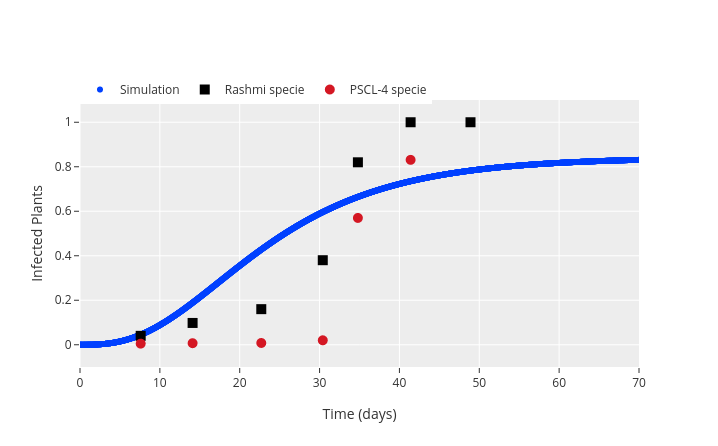
\includegraphics[scale=0.385, keepaspectratio]{%
	Figures/Tomato_with_data.png}
	\caption{Infected Plant population with two types of tomato species. The curve represent
	a susceptible variety of tomato the parameters are taking of deterministic case of table
	\autoref{tbl:value}, $\mathcal{R}^d_0>1$.
		\href{https://plotly.com/~AdrianSalcedo/24/}{
		https://plotly.com/~AdrianSalcedo/24/}}
	\label{fig:Deterministic_Infected_with_data}
\end{figure}
			
	\section{Stochastic extension}
		%
\info{Include references}
Following ideas from [referencia], we quantify uncertinity in replanting rate of
plants, and  died rate of vector, $r_1$, $r_2$ and $\gamma$, see
\autoref{tbl:deterministic_tbl}, we perturb parameters  $r_1 ,r_2$ and $\gamma$
with a Brownian process to obtain a stochastic differential equation(SDE). 
Here, the perturbation describe stochastic environmental noise on each population.
In symbols $ dB(t)=B(t+dt)-B(t)$ denotes the increment of a standard Wiener
process, thus we perturb potentially replanting $r_1$, $r_2$, and vector death
$\gamma$ in the infinitiesimal time interval $[t, t + dt)$ by
\begin{equation}
	\label{eqn::NoisePerturbation}
	\begin{aligned}
		{r}_1 dt \rightsquigarrow r_1 dt + \sigma_L dB_p(t),
		\\
		{r}_2 dt \rightsquigarrow r_2 dt + \sigma_I dB_p(t),
		\\
		\gamma dt \rightsquigarrow \gamma dt + \sigma_v dB_v(t).
	\end{aligned}
\end{equation}

	Note that right hand side of \autoref{eqn::NoisePerturbation}
	is a random perturbations of parameters
$r_1$, $r_2$, $\gamma$, with mean
$
	\EX{r_1 dt + \sigma_L dB_p(t)}
$
and variance 
\change{review ending lines}
$
	\VarX{r_1 dt + \sigma_L dB_p(t)} = \sigma_L^2dt
$, 
$
	\EX{\tilde{r}_2dt} = r_2dt
$ 
and
$
	\VarX{\tilde{r}_2dt} = \sigma_I^2dt
$ 
and 
$
	\EX{\tilde{\gamma}dt} = \gamma dt
$ and 
$
	\VarX{\tilde{\gamma}dt} = \sigma_v^2dt
$.
%
Thus, we establish an stochastic extension from deterministic tomato model 
\autoref{sys::DeterministicSystem} by the It\^{o} SDE

\begin{equation}
	\label{sys::StochasticSystem}
	\begin{aligned}
		d S_p &=
			\left(
				-\beta_p S_p \frac{I_v}{N_v} + r_1 L_p + r_2 I_p
			\right)dt 
			+ \frac{S_p(\sigma_L L_p
			+ 
			\sigma_I I_p)}{N_p}dB_p(t) 
		\\
		dL_p &=
			\left(
				\beta_p S_p \frac{I_v}{N_v} - b L_p - r_1 L_p
			\right) dt 
			- \sigma_L \frac{S_pL_p}{N_p} dB_p(t) 
		\\
		d I_p &=
			\left(
				b L_p - r_2 I_p
			\right) dt 
			- \sigma_I \frac{S_pI_p}{N_p} dB_p(t) 
		\\
		dS_v &=
			\left(
				-\beta_v S_v \frac{I_p}{N_p} - \gamma S_v  + (1-\theta) \mu
			\right)dt - \sigma_v S_v dB_v(t) 
		\\
		d I_v &=
			\left(
				\beta_v S_v \frac{I_p}{N_p} -\gamma I_v + \theta \mu
			\right) dt 
			- \sigma_v I_v dB_v(t),
			 \\
			S_p(0) &=S_{p0}, 
            L_p(0) = L_{p0},
            I_p(0) = I_{p0},
            \\
             S_v(0) &= S_{v0},
              I_v(0) = I_{v0}
	\end{aligned}
\end{equation}

	\section{Existence of a unique positive solution}
		\label{sec:solution_existence}
		%!TEX root = ../main.tex
Thereom 3.4 \cite[see][p. 58]{Mao2008} assures the existence of unique solution of 
\autoref{sys::StochasticSystem} in a compact interval. Since we study asymptotic behaviour, 
we have to assure the existence of unique-globally-positive invariant solution 
of SDE \autoref{sys::StochasticSystem}. The following result prove that this set is positive invariant.
%
%\info{Modify notation of invariant set}
\begin{theorem}\label{thm::existence-unique}
	For any initial values 
	$
		(S_p(0), L_p(0), I_p(0), S_v(0), I_v(0))^{\top}
		\in \Gamma
	$, 
	exists unique a.s. invariant global positive solution to SDE 
	\autoref{sys::StochasticSystem} in $\Gamma$, that is,
	\begin{equation*}
		\probX{
			(L_p(t), I_p(t), S_v(t), I_v(t)) 
			\in 
			\Gamma, \quad
			\forall t \geq 0
		} = 1.
	\end{equation*}
\end{theorem}
%
\begin{proof}
		Since the right hand side of system \autoref{sys::StochasticSystem} are quadratic, 
	linear and constants terms, this imply that they are locally Lipschitz. We 
	know by \cite[see][pp.300]{Mao2008}, that for any initial condition
	$
		(
			S_p(0),
			L_p(0),
			I_p(0),
			S_v (0),
			I_v(0)
		)^{\top} \in \Gamma
	$ 
	there is a unique maximal local solution 
	$(S_p(t), L_p(t), I_p(t), S_v(t), I_v(t))^{\top}$ 
	at $t\in [0,\tau_e)$, where 
	$\tau_e$ is the explosion time. Let $k_0>0$ be sufficiently large, and 
	define the stopping time
	\begin{multline}
		\label{eqn:invariatn_set}
		\tau_k = %
			\inf
			\left\{
				t \in [0,\tau_e)
				: 
				L_p(t) \notin 
					\left(
						\frac{1}{k_0},
					 N_p - \frac{1}{k_0}
					\right)		
			%\right.
			%\\
			%\left.
			 \bigcup 
				I_p(t)
				\notin
				\left(
					\frac{1}{k_0}, 
					N_p-\frac{1}{k_0}
				\right)
			\right.
			\\
			\bigcup
			\left.		
					I_v(t) 
					\notin
					\left(
						\frac{1}{k_0},
						N_v - \frac{1}{k_0}
					\right)
			\right\},
		\end{multline}
    Since $k\geq k_0$ and $\left(\frac{1}{k},N_{\bullet}-\frac{1}{k}\right)$ is a increasing by 
    the right side, we have $\tau_1\leq \tau_2\leq \dots \leq \tau_k \ldots$ and by definition
    $\tau_k\leq\tau_e$. Then $\tau_k\to \tau_{\infty}$. In other words, $\tau_\infty = \infty$ a.s. 
	implies
	\begin{equation}
		\label{eqn:invariance_prop}
		(
			S_p(t),
			L_p(t),
			I_p(t),
			S_v(t),
			I_v(t)
		)^{\top}\in \mathbf{E}
	\end{equation}
	 a.s. for all $t\geq 0$. Thus, 
	we  show that $\tau_\infty=\infty$ a.s. To this end,  we proceed
	by contradiction. Suppose that the above statement is false for a given 
	time $t$, then there is 
	a pair of constants $T>0$ and $\epsilon  \in (0,1)$  such that some 
	component from $L_p,I_p,I_v$, or $L_p$, get-outs from its corresponding 
	interval
	$$
	\left(
		\frac{1}{k_0}, 
	N_{\bullet} - \frac{1}{k_0}
	\right), 
	$$
	that is, %
	$
		\P[\tau_\infty\leq T]>\epsilon 
	$. 
	Hence, there is an integer $k_1\geq k_0$ such that
%	
	\begin{equation}\label{eqn::Probabilityoftau_k}
		\P[\tau_k\leq T]>\epsilon,
		\quad \forall k\geq k_1.
	\end{equation}
	
		Define a function $V_p:(0,N_p)\rightarrow \mathbb{R}_+$ by
%	
	\begin{equation*}
		V_p(x) := 
			\frac{1}{x} + 
			\frac{1}{N_p-x}.
	\end{equation*}
%	
	According to the diffusion operation $\mathcal{L}$
	see \autoref{eqn::DifussionOperator}. By diffusion operator, we have, for any 
	$t\in [0,T]$ and $k\geq k_1$ 
%
	\begin{align*}
		\mathcal{L}[V_p(L_p)] 
			=&	
				\left[
					-\frac{1}{L_p^2} + 
					\frac{1}{(N_p - L_p) ^ 2}
				\right]
				\left[
					\beta_p S_p 
					\frac{I_v}{N_v} - 
					(b + r_1) L_p\right]
				\\
			&+
				\frac{1}{2}
				\left[
					\frac{2}{L_p^3} + 
					\frac{2}{(N_p - L_p)^3}
				\right]
				\sigma_p ^ 2
				\frac{L_p^2 S_p^2}{N_p^2}.
			\\
	\end{align*}
%	
	Expanding each term, we have
	\begin{align*}
		\mathcal{L}[V_p(L_p)] 
			&=	
				-\beta_p \frac{S_p I_v}{L_p^2 N_v} + 
				\beta_p \frac{S_p I_v}{(N_p -L_p) ^ 2 N_v} + 
				\frac{(b + r_1)}{L_p} - 
				\frac{(b+r_1)L_p}{(N_p-L_p)^2}
				\\
			&+
				\left[
					\frac{1}{L_p^3} + 
					\frac{1}{(N_p-L_p)^3}
				\right]
				\sigma_p ^ 2
				\frac{L_p^2 S_p^2}{N_p^2}.
				\\
	\end{align*}
%	
	Dropping negative terms, we bound the above relation by
	\begin{align*}
		\mathcal{L}[V_p(L_p)] 
			&\leq	
				\beta_p 
				\frac{S_p}{(N_p - L_p) ^ 2} + 
				\frac{(b + r_1)}{L_p} + 
				\left[
					\frac{1}{L_p^3} + 
					\frac{1}{(N_p-L_p)^3}
				\right]
				\sigma_p ^ 2
				\frac{L_p ^ 2 S_p ^ 2}{N_p ^ 2}.
	\end{align*}
	Since $S_p\leq S_p+I_p\leq N_p-L_p$, we have $\frac{S_p}{N_p-L_p}\leq 1$, then
	%\info{Rewview this steap}
	\begin{align*}
		\mathcal{L}[V_p(L_p)] 
			&\leq		
				\frac{\beta_p}{N_p -L_p} + 
				\frac{(b + r_1)}{L_p} + 
				\sigma_p^2
				\left[
					\frac{1}{L_p} + 
					\frac{L_p^2}{N_p^2(N_p-L_p)}
				\right].
	\end{align*}
	And by $L_p\leq N_p$ we bound the diffusion operator as
	%\info{explain why}
	\begin{align*}
		\mathcal{L}[V_p(L_p)] 
			&\leq		
			\frac{b+r_1}{L_p} + 
			\frac{\beta_p}{N_p -L_p} +  
			\sigma_p^2
			\left[
				\frac{1}{L_p} + 
				\frac{1}{N_p-L_p}
			\right].
	\end{align*}
	%
	Now define $C := (b+r_1) \vee \beta_p +\sigma_p^2$, we obtain the 
	following inequality
	\begin{align}\label{eqn::BoundDiffusionOperator}
		\mathcal{L}[V(L_p)] 
			&\leq		
				C V_p(L_p).
	\end{align}
	
	By It\^{o}'s formula see Appendix A \autoref{eqn::Itoformula}, and applying
	\change{Fix appendix reference}
	expectation, we have, for any 
	$t \in [0,T]$ and $k\geq k_1$
	\begin{align*}
		\E V(L_p(t\wedge\tau_k)) &= 
			V(L_p(0)) + 
			\E 
				\int_{0}^{t\wedge\tau_k} \mathcal{L}[V(L_p(s))]
			ds.
	\end{align*}
	%
	By equation \autoref{eqn::BoundDiffusionOperator} and Fubini's Theorem, we have
	\begin{align*}
		\E V(L_p(t\wedge\tau_k)) 
			&\leq 
				V(L_p(0)) + 
				C
				\int_{0}^{t}
					\E V(L_p(s\wedge\tau_k))
				ds.
	\end{align*}
	Applying the Gronwall inequality yields that	
	\begin{align}\label{eqn::GronwallBound}
		\E V(L_p(t\wedge\tau_k))&\leq V(L_p(0))e^{CT}.
	\end{align}

		Set 
	$
		\Omega_k = \{\omega : \tau_k\leq T\}
	$ for $k\geq k_1$, note that by relation in 
	\autoref{eqn::Probabilityoftau_k}, 
	$
		\P(\Omega_k) >  \epsilon
	$. For every 
	$
		\omega \in \Omega_k
	$, we have 
	$
		L_p(t,\omega) \in 
		\left(
			\frac{1}{k_0}, N_p - 
			\frac{1}{k_0}
		\right) ^ {\complement}
	$, and hence
	\begin{align*}
		V_p(L_p(t,\omega))
			&=
				\frac{1}{L_p} + 
				\frac{1}{N_p-L_p}
			\\
			&\geq 
				k + 
				\frac{1}{
					N_p - \frac{1}{k}}
			\\
			& \geq k.
	\end{align*}
%	
	It follows from equation \autoref{eqn::GronwallBound}, that
	\begin{equation*}
		V_p(L_p(0)) e^{CT}
			\geq 
			\E 
			\left[
				\1{\Omega_k} (\omega)
				V_p(L_p(\tau_k,\omega))
			\right]
			\geq k
			\prob (\Omega_k)\geq \epsilon k.
	\end{equation*}
%
	Thus, letting $k\rightarrow \infty$ leads to the contradiction
	\begin{equation*}
		\infty>V_p(L_p(0))e^{CT}\geq \infty.	
	\end{equation*}
%
	Therefore we  have $\tau_\infty=\infty$ a.s., and the proof is 
	complete. \qed
\end{proof}

	\section{Disease extinction}
		\label{extinction}
		%!TEX root = ../main.tex
	In this section we will study when the disease can be extinguished, for 
this we will give the necessary conditions so that this phenomenon can occur 
through two different cases. The first case will be when due to the intensity 
of the noise.The theorem presented below shows that under conditions on the
parameters we can make the disease tend to become extinct.
%\change{Change definition to taalkabout FDE point}
\begin{definition}\label{def::ExponentialStability}
The free-disease fixed point of \autoref{sys::StochasticSystem} is said to be almost surely exponentially stable if
\begin{equation}\label{eqn::ExponentialStability}
		\limsup_{t \to \infty}
		\frac{1}{t}
		\ln(L_p + I_p) < 0 \text{ and }
		\limsup_{t \to \infty}
		\frac{1}{t}\ln(I_v)< 0\qquad\mbox{a.s.}
\end{equation}
\end{definition}

\begin{theorem}\label{thm::NoiseExtinction}
	Let	any initial condition $(S_p(0), L_p(0), I_p(0), S_v(0), I_v(0)) ^ \top \in \Gamma$. If
	\begin{align*}
		\frac{\beta_p ^ 2}{2\sigma_L ^ 2} + 
		\frac{r_2^2}{2\sigma_I^2} + 
		2 \beta_p - r_1 < 0,
		\qquad
		\frac{\beta_v^2}{2\sigma_v^2} + 
		\beta_v - \gamma + \theta \mu < 0,
	\end{align*}
	 then the disease will exponentially extinguish with probability one. That 
	 is, 
	\begin{equation*}
		\limsup_{t \to \infty}
		\frac{1}{t}
		\ln(L_p + I_p) < 0 \text{ and }
		\limsup_{t \to \infty}
		\frac{1}{t}\ln(I_v)< 0\qquad\mbox{a.s.}
	\end{equation*}
\end{theorem}
\begin{proof}
	The main idea is apply the It\^{o} formula to a conveniently function and 
	deduce conditions. Let 
	$
		V(S_p, L_p, I_p) = \ln(L_p + I_p)
	$, then the It\^{o} formula gives
	\begin{align*}
		d \ln(L_p+I_p) 
			=&
				\left(
					\frac{1}{L_p + I_p}
				\right)
				\left(
					\frac{\beta_p}{N_v^\infty} 
					S_p I_v - (b + r_1) L_p
					-\frac{1}{2}
					\sigma_L^2 \frac{L_p^2}{(L_p+I_p)^2}
				\right)dt
			\\
			&-
				\sigma_L \frac{L_p}{L_p+I_p}dB_p(t)\\
			&\leq 
				\left(
					\frac{1}{L_p+I_p}
				\right)
				\left(
					\beta_p S_p - (b + r_1) -
					\frac{1}{2}
					\sigma_L^2
					\frac{L_p^2}{(L_p+I_p)^2}
				\right)dt
			\\
			&-
				\sigma_L \frac{L_p}{L_p + I_p} dB_p(t).
			\\
	\end{align*}
	Let $x:=\frac{L_p}{L_p + I_p}$, then
		\begin{align*}
		d \ln(L_p + I_p) 
			&\leq 
				\left(
					\beta_p 
					\frac{S_p}{L_p + I_p} - 
					(b + r_1) - 
					\frac{1}{2}
					\sigma_L ^ 2 x^2
				\right)dt - \sigma_L x dB_p(t)
			\\
			&\leq
				\left(\beta_p
					\frac{N_p}{L_p + I_p} - (b+r_1) - 
					\frac{1}{2} 
					\sigma_L^2 x^2
				\right) dt - 
				\sigma_L xdB_p(t)
			\\
			&\leq
				\left(
					\beta_p x + 2\beta_p - 
					(b + r_1) - 
					\frac{1}{2}
					\sigma_L ^ 2 x^2
				\right) dt - 
				\sigma_L xdB_p(t)
			\\
			&=
				\left(
					-\frac{1}{2}
					\sigma_L ^ 2 x ^ 2 + 
					\beta_p x + 2 \beta_p - 
					(b + r_1)
				\right) dt -\sigma_L x 
				dB_p(t).			
	\end{align*}
	Hence,
	\begin{align*}
		\ln(L_p+I_p)
			&\leq
				-\frac{\sigma_L ^ 2}{2}
				\int_{0} ^ {t}
					\left[
						\left(
							x - 
							\frac{\beta_p}{\sigma_L ^ 2}
						\right) ^ 2 + 
						\frac{\beta_p ^ 2}{2 \sigma_L ^ 2} + 
						2 \beta_p - (b + r_1)
					\right] du
				\\
			&-
				\int_{0} ^ {t}
					\sigma_L x dB_p(u) + 
					\ln(L_p(0) + I_p(0)),
	\end{align*}
	which implies,
	\begin{equation}
	\label{eqn::ItoForBound}
		\begin{aligned}
			\frac{1}{t}\ln(L_p+I_p) 
				&\leq
					-\frac{\sigma_L^2}{2t}
					\int_{0}^{t}
					\left(
						x - 
						\frac{\beta_p}{\sigma_L^2}
					\right) ^ 2 du + 
					\frac{\beta_p^2}{2\sigma_L^2} - 
					(b + r_1) + 2\beta_p
				\\
				&-
					\frac{1}{t}
					\int_{0}^{t}
					\sigma_L x dB_p(u) + 
					\frac{1}{t} \ln(S_p(0)+L_p(0)+I_p(0)),
		\end{aligned}
	\end{equation}
	let 
	$$
	M_t :=
		\frac{1}{t}
		\int_{0}^{t}
			\sigma_L x dB_p(t) + 
			\frac{1}{t} \ln(L_p(0)+I_p(0)) .
	$$ 
	Since the integral in the term $M_t$ is a martingale, the strong law of
	large numbers for martingales \cite[see][Theorem 3.4, pp.12]{Mao2008}, implies that
	\begin{equation*}
		\lim
		\limits_{t \to \infty} M_t = 0\,\,
		\mbox{a.s.}
	\end{equation*}
	Thus, from relation \autoref{eqn::ItoForBound} we obtain
	\begin{align}
		\label{eqn::Bound1}
		\limsup_{t\infty \to \infty}
		\frac{1}{t}
		\ln(L_p + I_p) < 
			\frac{\beta_p^2}{2\sigma_L^2} +
			2\beta_p - (b + r_1)
	\end{align}
	A similar argument also shows that
	\begin{align}\label{eqn::Bound2}
		\limsup_{t\infty \to \infty}
		\frac{1}{t}
		\ln(L_p + I_p) < 
		\frac{r_2 ^ 2}{2 \sigma_I ^ 2} + b
	\end{align}
%
	Through by \autoref{eqn::Bound1} and \autoref{eqn::Bound2}, we obtain
%	
	\begin{align*}
		\limsup_{t\infty \to \infty}
		\frac{1}{t}
		\ln(L_p + I_p) 
			< 
			\frac{\beta_p^2}{2\sigma_L^2} + 
			\frac{r_2^2}{2 \sigma_I ^ 2} +	
			2\beta_p - r_1
	\end{align*}
	and for infected vector we obtain
	\begin{align*}
		\limsup_{t\infty \to \infty}
		\frac{1}{t}
		\ln(I_v) 
			< 
			\frac{\beta_v^2}{2\sigma_v^2} 
			+ 
			\beta_v - \gamma + \theta \mu
	\end{align*}
	\qed
\end{proof}
%
\begin{remark}
\autoref{thm::NoiseExtinction} shows that, under certain conditions on the
parameters can cause disease exponentially towards zero whenever the noise
intensity is large enough.
\end{remark}

To define the stochastic reproductive number we will use techniques similar to
those used in\cite{Agarwal2019}, in which, by means of algebraic procedures,
this parameter can be defined. 

To define the basic stochastic reproductive number, let's define 
$ r = \max \{r_1, r_2 \}$. 
Then the basic reproductive number of the system \autoref{sys::StochasticSystem}
is defined as

\begin{equation}\label{eqn::StochasticBRN}
	\mathcal{R}_0 ^ s =
		\frac{\beta_p \beta_v}{\gamma r}.
\end{equation}
%
The following theorem proves that under $\mathcal{R}^s_0<1$, the infected plants
and vectors tends to zero.
%\change{Rewrite according to the above notation}
\begin{theorem}
	\label{thm::Rs0Extinction}
	Let $(S_p(t),L_p(t),I_p(t),I_v(t))^\top$ 
	be the solution of SDE \autoref{sys::StochasticSystem} with initial values 
	$
		(S_p(0),L_p(0),I_p(0),I_v(0))^\top \in \Gamma
	$. 
	If $0\leq \mathcal{R}^s_0<1$, 
	then the following conditions holds
	\begin{align*}
		\lim
		\limits_{t\to \infty}
		\frac{1}{t}
		\mathbb{E}
		\int_{0}^{t}
			\left[
				r
				[\mathcal{R}^s_0 - 1]
				I_p - r S_p
				\left(
					1 - \frac{S^0_p}{S_p}
				\right) ^ 2 - 
				r L_p - 
				\frac{\beta_p\beta_v}{\gamma} 
				I_v I_p
			\right] dr 
			\leq \frac{1}{2} \sigma_p^ 2 N_p,\, a.s.,
	\end{align*}
	namely, the infected individual tends to zero exponentially a.s, i.e the 
	disease will die out with probability one.
\end{theorem}
%
\begin{proof}
	The proof consist verify the hypotheses of Khasminskii Theorem 
	\change{Fix citation}
	\info{Write Khasminskii Theorem in appendix}
	\cite{Agarwal2019} for 
	the Lyapunov function
	%
	\begin{align*}
		V(S_p, L_p, I_p, S_v, I_v) 
			=& 
				\left(
					S_p - N_p - N_p 
					\ln 
					\frac{S_p}{N_p}
				\right) + 
				L_p + I_p + 
				\frac{\beta_p N_p}{\gamma N^\infty_v} I_v
			\\
			&+
				\left(
					S_v - N_v - N_v 
					\ln
					\frac{S_v}{N_v}
				\right).
	\end{align*}
	%
	Let $f$, $g$ respectively be the drift and diffusion of SDE 
	\autoref{sys::StochasticSystem}. Applying the diffusion operator
	$\mathcal{L}$ we have
	%
	\begin{equation}\label{eqn::LyapunovFunction}
		\begin{aligned}
			V_x f 
				&\leq
					\left(
						1 - 
						\frac{N_p}{S_p}
					\right)
					\left(
						-
						\frac{\beta_p}{N^\infty_v} S_p I_v + 
						r N_p - r S_p
					\right) + 
					\frac{\beta_p}{N^\infty_v} S_p I_v - 
					(b + r) L_p
				\\
				&+
					b L_p - r I_p + 
					\left(
						1 - 
						\frac{N_v}{S_v}
					\right)
					\left( 
						-\frac{\beta_v}{N_p} S_v I_p - 
						\gamma S_v + 
						(1 - \theta) \mu 
					\right)
				\\
				&+
					\frac{\beta_p N_p}{\gamma N ^ \infty_v}
					\left(
						\frac{\beta_v S_v}{N_p}
						I_p - \gamma I_v + 
						\theta \mu
					\right)  \ .
		\end{aligned}
	\end{equation}
	Expanded the term $\left(
				1 - \frac{N_p}{S_p}
			\right)
			\left(
				-\frac{\beta_p}{N^\infty_v} S_p I_v +
				r N_p - r S_p
			\right)$ 
			of \autoref{eqn::LyapunovFunction} and factoring the term $S_p$,
			we obtain
	\begin{equation}
		\label{theorem2term1}
		\begin{aligned}
			\left(
				1 - \frac{N_p}{S_p}
			\right)
			&
			\left(
				-\frac{\beta_p}{N^\infty_v} S_p I_v +
				r N_p - r S_p
			\right) 	
			\\
			&=
				\left(
						1 - \frac{N_p}{S_p}
					\right)
					\left(- r S_p 
						\left(
							1 - \frac{N_p}{S_p}
						\right) - 
						\frac{\beta_p}{N^\infty_v} S_p I_v
					\right)
			\\
			&=
				- r S_p 
				\left(
					1 - 
					\frac{N_p}{S_p}
				\right) ^ 2 - 
				\frac{\beta_p}{N ^ \infty_v} S_p I_v + 
				\frac{\beta_p}{N ^ \infty_v} N_p I_v .
		\end{aligned}
	\end{equation}
	%\improvement{rewrite}
	For the term $\left(
				1 - 
				\frac{N_v}{S_v}
			\right)
			\left(
				-\frac{\beta_v}{N_p} S_v I_p - 
				\gamma S_v + 
				(1 - \theta) \mu 
			\right) $,
			since $\theta\in [0,1]$ and $(1-\theta)\mu\leq \gamma N_v$
			we bound by the following
	\begin{equation}\label{theorem2term2}
		\begin{aligned}
			\left(
				1 - 
				\frac{N_v}{S_v}
			\right)
			&
			\left(
				-\frac{\beta_v}{N_p} S_v I_p - 
				\gamma S_v + 
				(1 - \theta) \mu 
			\right) 
			\\
			&
			\leq
				\left(
					1 - \frac{N_v}{S_v}
				\right)
				\left(- 
					\frac{\beta_v}{N_p} S_v I_p -
					\gamma S_v +\gamma N_v
				\right)
			\\
			&\leq
				\left(
					1 - \frac{N_v}{S_v}
				\right)
				\left(-
					\gamma S_v
					\left(
						1 - 
						\frac{N_v}{S_v}
					\right) -
					\frac{\beta_v}{N_p} S_v I_p
				\right)
			\\
			&\leq
				-\gamma S_v 
				\left(
					1- 
					\frac{N_v}{S_v}
				\right) ^ 2 - 
				\frac{\beta_v}{N_p} S_v I_p + 
				\frac{\beta_v}{N_p} N_v I_p \ .
		\end{aligned}
	\end{equation}
	Same way from above calculation, and since 
	$\theta \mu\leq \theta\gamma N_v$, we obtain
	\begin{equation}
		\label{theorem2term3}
		\begin{aligned}
			\frac{\beta_p N_p}{\gamma N^\infty_v}
			\left(
				\frac{\beta_v S_v}{N_p} I_p- 
				\gamma I_v + \theta \mu
			\right)
			&\leq
				\frac{\beta_p N_p}{\gamma N^\infty_v}
				\left(
					\frac{\beta_v S_v}{N_p} I_p -
					\gamma I_v + 
					\theta \gamma N_v
				\right) 
			\\
			&\leq
				\frac{\beta_p \beta_v S_v I_p}{\gamma N_v} - 
				\frac{\beta_p N_p}{ N^\infty_v} I_v + 
				\beta_p \theta N_p.
		\end{aligned}
	\end{equation}
	\begin{align*}
		V_x f 
			& \leq
				- r S_p 
				\left(
					1 - 
					\frac{N_p}{S_p}
				\right) ^ 2 + 
				\left[
					\frac{\beta_p}{N^\infty_v} N_p - 
					\frac{\beta_p N_p}{ N^\infty_v}
				\right] I_v - 
				r (L_p + I_p)
			\\
				& -
				\gamma S_v
				\left(
					1 - 
					\frac{N_v}{S_v}
				\right) ^ 2 - 
				\frac{\beta_v}{N_p} S_v I_p + 
				\frac{\beta_v}{N_p} N_v I_p
			\\
				& +
				\frac{\beta_p\beta_v S_v I_p}{\gamma N_v} + 
				\beta_p \theta N_p \ .
	\end{align*}
	%
	Moreover, since $S_v+I_v\leq N_v$, we can obtain the following relation
	%
	\begin{align*}
		V_x f 
			\leq &
				- r S_p 
				\left(
					1 - 
					\frac{N_p}{S_p}
				\right) ^ 2 - 
				r (L_p + I_p)
			\\
			&-
				\gamma S_v
				\left(1 - 
					\frac{N_v}{S_v}
				\right) ^ 2 + 
				\frac{\beta_v}{N_p} I_v I_p
			\\
			&+
				\frac{\beta_p\beta_v I_p}{\gamma} - 
				\frac{\beta_p\beta_v I_v I_p}{\gamma N_v} + 
				\beta_p \theta N_p \ .
	\end{align*}
%
	Expressing the right hand side of above equation in term of the basic 
	reproductive number, $\mathcal{R}^s_0$ we get
	\begin{align*}
		V_x f 
			&\leq
				-rS_p 
				\left(
					1 - 
					\frac{S_p^0}{S_p}
				\right) ^ 2 -
				\gamma S_v
				\left(
					1 - 
					\frac{N_v}{S_v}
				\right) ^ 2 - 
				r L_p - r
				\left[
					1 - \mathcal{R}^s_0
				\right] I_p
			\\
			&-
				\left[
					\frac{\beta_p\beta_v}{\gamma N^\infty_v} - 
					\frac{\beta_v}{N_p} 
				\right] I_v I_p - 
				\frac{\beta_v}{N_p} S_v I_p + 
				\beta_p \theta N_p \ .
	\end{align*}
	%
	Moreover,
	%
	\begin{align*}
		\frac{1}{2}
		\trace(g ^ TV_{xx} g) 
		&=
		\frac{1}{2} 
		\frac{
			\left(
				 \sigma_L L_p + \sigma_I I_p
			\right) ^ 2
		}{N_p} 
		+ 
		\frac{1}{2} \sigma_v ^ 2 N_v,
	\end{align*}
	%
	define $\sigma_p = \max\{\sigma_L,\sigma_I\}$, then
	
		\begin{align*}
		\frac{1}{2}
		\trace(g ^ TV_{xx} g) 
		&\leq
		\frac{1}{2} 
		\sigma_p ^ 2 N_p +  
		\frac{1}{2} \sigma_v ^ 2 N_v \ .
	\end{align*}
	
	The stochastic terms are not necessary, because they do a martingale process
	and by the Strong law of large numbers, Theorem 3.4 
	\cite[see][pp. 12]{Mao2008},when we use integral and expectation they
	vanishing. Incorporation all terms calculate above, we obtain
	\begin{align*}
	 	\mathcal{L}V(X) 
			&\leq
				-r S_p
				\left(
					1 -\frac{S_p^0}{S_p}
				\right) ^ 2 - 
				\gamma S_v
				\left(
					1 - 
					\frac{N_v}{S_v}
				\right) ^ 2 - 
				r L_p - r 
				\left[
					1 - \mathcal{R}^s_0
				\right] I_p
			\\
			&-
				\left[
					\frac{\beta_p \beta_v}{\gamma N ^ \infty_v} - 
					\frac{\beta_v}{N_p}
				\right] I_v I_p - 
				\frac{\beta_v}{N_p} S_v I_p + 
				\beta_p \theta N_p + 
				\frac{1}{2} 
				\sigma_p ^ 2 N_p + 
				\frac{1}{2}
				\sigma_v^2 N_v\ .
			\\
	\end{align*}
	%
	Define 
	$
		\sigma_{p,v}:= 
			\beta_p \theta N_p + 
			\frac{1}{2} 
			\sigma_p ^ 2 N_p +  
			\frac{1}{2} \sigma_v ^ 2 N_v
	$, then
	\begin{align*}
		\mathcal{L}V(X) 
			&\leq
				-r S_p
				\left(
					1 - 
					\frac{S_p^0}{S_p}
				\right) ^ 2 - 
				\gamma S_v
				\left( 1 -
					\frac{N_v}{S_v}
				\right) ^ 2 - r L_p - r 
				\left[
					1 - \mathcal{R}^s_0
				\right] I_p
			\\
			&-
				\left[
					\frac{\beta_p\beta_v}{\gamma N^\infty_v} - 
					\frac{\beta_v}{N_p}
				\right] I_v I_p - 
				\frac{\beta_v}{N_p} S_v I_p + 
				\sigma_{p,v} \ .
	\end{align*}
	%
	Since $V(x)\geq 0$, using the integral form of It\^{o}'s formula and 
	taking expectation yields
	\begin{align*}
		0 
		&\leq
			\mathbb{E}V(t) - 
			\mathbb{E} V(0)
			\leq
			\mathbb{E}
			\int_{0} ^ {t}
				\mathcal{L} V(X(s)) ds
			\\
		&\leq
			-\mathbb{E}
			\int_{0} ^ {t}
			\left[
				rS_p 
				\left(
					1 - \frac{S_p^0}{S_p}
				\right)^2 + 
				\gamma S_v
				\left(1 - 
					\frac{N_v}{S_v}
				\right) ^ 2 + 
				r L_p + 
				r 
				\left[
					1 - \mathcal{R} ^ s _ 0
				\right] I_p 
			\right.
		\\
		&+
			\left.
				\left[
					\frac{\beta_p\beta_v}{\gamma N^\infty_v} + 
					\frac{\beta_v}{N_p}
				\right] I_v I_p + 
				\frac{\beta_v}{N_p} S_v I_p - 
				\sigma_{p,v}
			\right] ds \ .
	\end{align*}
%
	Therefore,
%	
	\begin{align*}
		\frac{1}{t}
		\mathbb{E}
			&\int_{0}^{t}
				\left[
					rS_p 
					\left(
						1 - \frac{S_p^0}{S_p}
					\right) ^ 2 +
					\gamma S_v
					\left(
						1 - \frac{N_v}{S_v}
					\right) ^ 2 + 
					r L_p + 
					r 
					\left[
						1 - \mathcal{R} ^ s_ 0
					\right]I_p 
				\right.
			\\
			&+
				\left.
					\left[
						\frac{\beta_p \beta_v}{\gamma N ^ \infty_v} + 
						\frac{\beta_v}{N_p}
					\right] I_v I_p + 
					\frac{\beta_v}{N_p}S_vI_p
				\right] ds 
				\leq
				\sigma_{p,v} \ .
	\end{align*}
	This implies that,
	\begin{align*}
		\lim\limits_{t\to \infty}
		\frac{1}{t} \mathbb{E}
			&
			\int_{0}^{t}
			\left[
				r S_p
				\left(
					1 - 
					\frac{S_p^0}{S_p}
				\right) ^ 2 + 
				\gamma S_v
				\left(
					1 - \frac{N_v}{S_v}
				\right) ^ 2 + 
				r L_p + 
				r 
				\left[
					1 - \mathcal{R} ^ s _ 0
				\right] I_p 
			\right.
		\\
		&+
		\left.
			\left[
				\frac{\beta_p \beta_v}{\gamma N ^ \infty_v} + 
				\frac{\beta_v}{N_p}
			\right] I_v I_p + 
			\frac{\beta_v}{N_p}S_v I_p
		\right] ds 
		\leq 
		\sigma_{p,v}.
	\end{align*}
	%
	Taking 
	$\theta$, $\sigma_p$, and $\sigma_v$ such that $0<\sigma_{p,v}< 1$, we 
	have
	\begin{multline*}
		\lim%
		\limits_{t\to \infty}
		\frac{1}{t}
		\log
		\mathbb{E}
		\int_{0} ^ {t}
			%
			\left[
				r S_p
				\left(
					1-
					\frac{S_p ^ 0}{S_p}
				\right) ^ 2 +
			\right.
			%
			\gamma S_v
			\left(
				1 - 
				\frac{N_v }{ S_v}
			\right) ^ 2 + 
			%& 
			r L_p + r
			\left[
				1 - \mathcal{R}^s_0
			\right] I_p 
		\\
			 +
			%	
			\left(
				\frac{\beta_p\beta_v}{\gamma N^\infty_v} + 
				\frac{\beta_v}{N_p}
			\right) I_v I_p + 
		 %\\	
			%& 
			\left.
				\frac{\beta_v}{N_p} S_v I_p
			\right] 
			ds \leq 
			\log 
				\sigma_{p,v} <0 \ .
	\end{multline*}
	Therefore,
	\begin{multline*}
		\lim
		\limits_{t\to\infty}
		\mathbb{E}
			\int_{0} ^ {t}
		 		\left[ 
		 			r S_p
		 			\left(
		 				1 - 
		 				\frac{S_p^0}{S_p}
		 			\right)^ 2 +
		 		\right.
		 		\gamma S_v
		 		\left(
		 			1 - 
		 			\frac{N_v}{S_v}
		 		\right) ^ 2 + 	
				r L_p 
		 			+ 
		 			r
		 			\left[
		 				1 - \mathcal{R}^s_0
		 			\right] I_p 
				+
				\\
				\left.
					\left[
						\frac{\beta_p \beta_v}{\gamma N ^ \infty_v} + 
						\frac{\beta_v}{N_p}
					\right] I_v I_p + 
					\frac{\beta_v}{N_p} S_v I_p
				\right] 
				ds 
				\leq
				\lim
				\limits_{t\to \infty}
					e^{\sigma_{p,v} t } = 0 \ .
	\end{multline*}
%		\improvement{rewrite}
Letting $t \to \infty$ we obtain
	\begin{align*}
		\lim\limits_{t \to\infty}
			(S_p, L_p, I_p, S_v, I_v )^{\top}_{t}
			=
			(N_p, 0, 0, N_v, 0)
	\end{align*}
		exponentially a.s. \qed
\end{proof}
\begin{remark}
	Theorem \ref{thm::Rs0Extinction} shows that, if the basic stochastic
	reproductive number $\mathcal{R}^s_0$ is less than one, we have the 
	solutions $X(t)=(S_p (t), L_p (t), (t ) I_p (t), S_v (t), I_v (t))^{\top}$ 
	tend to the equilibrium point $(N_p, 0,0, N_v^{\infty}, 0)^{\top}$, 
	when $t\rightarrow \infty$.
\end{remark}
	\section{Persistence}
		\label{sec:persistence}
		%!TEX root = ../main.tex

	In the case of deterministic models, one of the problems taken into
account is to determine under what conditions the endemic equilibrium point is 
attractor or asymptotically stable. In the case of stochastic models, said 
endemic equilibrium point is not an equilibrium point. To determinate the 
persistence in the stochastic cases, we use the following definition.

\change{Rewrite according to 
    oscillations around deterministic endemic fixed point
}
	So how do we determine if the disease is going to persist? In this section 
we will give the conditions under which the difference between the solution of 
the system \autoref{sys::StochasticSystem} and $ (S_p^{**}, L_p^{**}, I_p^{**}, S_v^{**}, I_v^{**})^\top$ is 
small if the noise is weak, reflecting that the disease is prevalent.

First we prove that each of the populations is bounded superiorly. Then, using the upper bound and
hypothesis 2 we will prove that the populations are lower bound. 
And let's finish by applying the definition of persistence.

We use the definition given in \cite{Zhao2015a} to prove the persistence of the disease.
\begin{definition}{\cite[][Def. *.*]{Zhao2015a}}
\label{def::persistence}
	Let $x = \{S_p,L_p,I_p,S_v,I_v\}$ be the solution of 
	system \autoref{sys::StochasticSystem}. 
	We said that this solution process is persistent in mean if	
	\begin{equation}
	    \liminf_{
	    	t \to
	    	\infty
	    }
	    \frac{1}{t}
	    \int_0^t x(r) dr >0,
	    \qquad a.s.
    \end{equation}
\end{definition}
For establish the persistent of the endemic equilibrium point of
\autoref{sys::StochasticSystem}, we need consider the opposite conditions
of \autoref{thm::NoiseExtinction}.
Our analysis require the following hypothesis.
\change{Justify the intention of next hypothesis.}

\begin{hyp}\label{eqn::NoiseBreak}
	\item
	According to \autoref{thm::NoiseExtinction}, 
	we need consider  
	$$
		\frac{\beta_p^2+r^2}{2 \sigma_p^2} + 
		2\beta_p - r>0,
	$$ 
    \item
	and
	$$
		\frac{\beta_v^2}{2 \sigma_v^2}+\beta_v-\gamma +\theta\mu>0.
	$$
\end{hyp}

Note, from \autoref{eqn::DeterministicBRN} we know that
$\mathcal{R}^d_0<\mathcal{R}_0 ^ s $. So we have the relation 
$\mathcal{R}_0 ^s <1 $ implies that $\mathcal{R}_0 ^ d<1$, and 
$\mathcal{R}_0 ^d >1 $ implies that $\mathcal{R}_0 ^ s>1$. The following 
Theorem gives a upper bound for \autoref{sys::StochasticSystem}.
%
\begin{theorem}
	\label{thm::UpperBound}
	Let $\mathcal{R}^s_0>1$ and condition \autoref{eqn::NoiseBreak} hold. 
	Consider the endemic deterministic fixed point 
	$(S_p^{**},L_p^{**},I_p^{**},S_v^{**},I_v^{**})^\top$. Then 
	\begin{equation}\label{eqn::UP-1}
		\begin{aligned}
			&\limsup\limits_{t \rightarrow 	\infty}
			\frac{1}{t}
			\int_{0}^{t}( r
				\left(
					1 - 2 \rho_1
				\right)
				\left(
					(S_p - S_p^{**}) ^ 2 + 
					(L_p - L_p^{**}) ^ 2 + 
					(I_p - I_p^{**}) ^ 2
				\right)
			\\
			&+
				\gamma
				\left(
					1 - 2 \rho_2
				\right)
				(S_v - S_v^{**}) ^ 2 - 
				\gamma
				\left(
					1 - 
					\frac{1}{4 \rho_2}
				\right)
				(I_v - I_v^{**})^2)ds
			\\
			&\leq
				K_2
				\alpha_1 + K_1
				\alpha_2 + 
				\frac{1}{2}
				\left(
					\sigma_p ^ 2
					( L_p ^{**}K_1 + I_p ^{**} K_2 + 2N_p^2)
					+3 N_v^2 \sigma_v^2
				\right)
				\qquad\mbox{a.s.}
		\end{aligned}
	\end{equation}
%
	where 
	$
		K_1 = \frac{N_p^2}{L_p^{**}}
	$, 
	$
		K_2 = \frac{N_p^2}{I_p^{**}}
	$, 
	$
		\rho_1 \in (0, \frac{1}{2})
	$ and 
	$
		\rho_2\in (\frac{1}{4}, \frac{1}{2})
	$.
\end{theorem}
%
\begin{proof}
	By hypothesis 
	$
		(S_p^{**}, L_p^{**}, I_p^{**}, S_v^{**}, I_v^{**}) ^ \top
	$ is the endemic equilibrium of \autoref{sys::DeterministicSystem}, we have
	\begin{equation}
		\begin{aligned}
			rN_p
				&=
					rS_p^{**} + 
					\frac{\beta_p}{N_v}S_p^{**}I_v^{**},
					\quad\quad 
					\frac{\beta_p}{N_v}S_p^{**}I_v^{**} = (b+r)L_p^{**},
			\\
			bL_p^{**}
				&=
					rI_p^{**}, 
					\quad\quad 
					(1-\theta)
					\mu = \frac{\beta_v}{N_p}S_v^{**}I_p^{**}+\gamma S_v^{**},
			\\
					\theta\mu &= 
					\gamma I_v^{**} -\frac{\beta_v}{N_p}S_v^{**}I_p^{**}.
		\end{aligned}
	\end{equation}
	Let consider the following Lyapunov function
	\begin{align*}
		V(S_p,L_p,&I_p,S_v,I_v) = 
				K_1
				\left(
					L_p - L_p^{**} - 
					L_p^{**}\log
					\left(
						\frac{L_p}{L_p^{**}}
					\right)
				\right) 
				\\
				&+ 
				 K_2
				\left(
				 	I_p - I_p^{**} - I_p^{**} 
				 	\log
					\left(
						\frac{I_p}{I_p^{**}}
				 	\right)
				\right)
			\\
				&+
				\frac{1}{2}
				\left[
					(S_p - S_p^{**}) + 
					(L_p - L_p^{**}) + 
					(I_p - I_p^{**})
				\right]^2 
				\\
				&+ 
				\frac{1}{2}
				\left[
					(S_v - S_v^{**}) + 
					(I_v - I_v^{**})
				\right]^2		
	\end{align*}
	We can rename the Lyapunov function as the follows
	\begin{equation}
		V(S_p,L_p,I_p,S_v,I_v)= K_1V_1+K_2V_2+V_3+V_4,
	\end{equation}
%
	and we work with each $V_i$. For $V_1$, we have
	\begin{align*}
		\mathcal{L} V_1 
			&= 
				\left(
					1 - 
					\frac{L_P^{**}}{L_p}
				\right)
				\left(
					\frac{\beta_p}{N_v}S_pI_v - 
					(b+r) L_p
				\right) + 
				\frac{1}{2}
				\frac{\sigma_p^2S_p^2L_p^{**}}{N_p^2}
			\\
			&=
				\left(
					1 - \frac{L_P^{**}}{L_p}
				\right)
				\left(
					\frac{\beta_p}{N_v} S_pI_v - 
					\frac{\beta_p}{N_v} S_p ^{**} I_v ^{**} 
					\frac{L_p}{L_p^{**}}
				\right) + 
				\frac{1}{2}
				\frac{\sigma_p^2S_p^2L_p^{**}}{N_p^2}
			\\
			&=
				\frac{\beta_p}{N_v}
				\left(
					1 - 
					\frac{L_P^{**}}{L_p}
				\right)
				\left(S_pI_v - 
					\frac{S_p^{**}I_v^{**}L_p}{L_p^{**}}
				\right) + 
				\frac{1}{2}
				\frac{\sigma_p^2S_p^2L_p^{**}}{N_p^2}
			\\
			&=
				\frac{\beta_p}{L_pN_v}
				\left(
					L_p - L_p^{**}
				\right)
				\left(
					S_pI_v - S_p ^{**} I_v^{**}
					\frac{L_p}{L_p^*}
				\right) + 
				\frac{1}{2}
				\frac{\sigma_p^2 S_p^2 L_p^{**}}{N_p^2}.
	\end{align*}
%
Now, for $V_2$ we have
%
	\begin{align*}
		\mathcal{L}V_2 
			&= 
				\left(
					1 - 
					\frac{I_P^{**}}{I_p}
				\right)
				\left(
					bL_p - r I_p 
				\right) + 
				\frac{1}{2}
				\frac{\sigma_p^2 S_p^2 I_p^{**}}{N_p^2}
			\\
			&= 
				\frac{1}{I_p}
				(I_p-I_p^{**})
				\left(
					\frac{rI_p^{**}}{L_p^{**}} - 
					rI_p
				\right) + 
				\frac{1}{2}
				\frac{\sigma_p^2 S_p^2 I_p^{**}}{N_p^2}
			\\
			&=
				-\frac{r}{I_p} (I_p - I_p ^{**})
				\left(I_p - \frac{I_p ^{**}}{L_p^{**}}
				\right) + 
				\frac{1}{2} 
				\frac{\sigma_p^2 S_p^2 I_p ^{**}}{N_p^2}.
	\end{align*}
	%
	For $V_3$, we obtain
%	\change{fix underfull, define $x-x^{**}$}
	\begin{align*}
		\mathcal{L}V_3
			&= 
				\left[
					(S_p - S_p ^{**} ) + 
					(L_p - L_p ^{**}) +
					(I_p - I_p ^{**})
				\right]
				\left(
					-\frac{\beta_p}{N_v}S_pI_v + 
					r N_p - rS_p 
				\right.\\
			&+
				\left.
					\frac{\beta_p}{N_v} 
					S_pI_v - (b+r)L_p + bL_p-rI_p
				\right) + 
				\sigma_p^2N_p^2
				\\
			&= 
				\left[
					(S_p - S_p^{**}) + 
					(L_p - L_p^{**}) + 
					(I_p - I_p^{**})
				\right]
				( r N_p - r S_p - r L_p - r I_p)
			\\
				& +
				\sigma_p^2N_p^2
			\\
			&=
				\left[
					(S_p - S_p ^{**}) + 
					(L_p - L_p ^{**}) + 
					(I_p - I_p^{**})
				\right]
				( r I_p ^{**} + r L_p^{**} + rS_p^{**} - rS_p 
				\\
				&-
				r L_p-r I_p)
				+ \sigma_p^2 N_p^2
			\\
			&=
				\left[
					(S_p - S_p ^{**}) + 
					(L_p - L_p ^{**}) +
					(I_p - I_p ^{**})
				\right]
				\\
				&\left[
					-r (S_p - S_p ^{**}) -
					r (L_p - L_p^{**}) 
					-r(I_p-I_p^{**})
				\right]
			+ 
				\sigma_p^2 N_p^2
			\\
			&=
				-r
				\left[
					(S_p - S_p ^{**}) + 
					(L_p - L_p ^{**}) +
					(I_p - I_p^{**})
				\right] ^ 2 + 
				\sigma_p^2 N_p^2.
	\end{align*}
	%
	For the last function $V_4$, we have
	%
	\begin{align*}
		\mathcal{L}V_4
			&= 
				\left[
					(S_v - S_v ^{**}) + 
					(I_v - I_v ^{**})
				\right]
				\left( - 
					\frac{\beta_v}{N_p} S_vI_p -
					\gamma S_v + 
					(1 - \theta) 
					\mu 
				\right.\\
			&+
				\left.
					\frac{\beta_v}{N_p}
					S_v I_p - 
					\gamma I_v + 
					\theta \mu 
				\right) + 
				\frac{3}{2}
				\sigma_v ^ 2 N_v ^ 2
				\\
			&=
				\left[
					(S_v - S_v^{**}) + 
					(I_v - I_v^{**})
				\right]
				(-\gamma S_v + \gamma S_v^{**} - \gamma I_v + \gamma I_v^{**}) + 
				\frac{3}{2}
				\sigma_v ^ 2 N_v ^ 2
			\\
			&=
				\left[
					(S_v - S_v ^{**}) + 
					(I_v - I_v ^{**})
				\right]
				\left[
					-\gamma (S_v - S_v^{**})
					-\gamma (I_v - I_v^{**})
				\right] + 
				\frac{3}{2}
				\sigma_v ^ 2 N_v ^ 2
				\\
			&=
				-\gamma 
				\left[
					(S_v - S_v ^{**}) + 
					(I_v - I_v^{**})
				\right] ^2 + 
				\frac{3}{2}
				\sigma_v ^2 N_v^2.
	\end{align*}
	%
	Then, we bound the diffusion operator as follows
	%
	\begin{align*}
		\mathcal{L}V 
			&\leq 
				-r 
				\left[
					(S_p - S_p ^{**}) + 
					(L_p - L_p ^{**}) +
					(I_p - I_p ^{**})
				\right] ^2 - 
				\gamma 
				\left[
					(S_v - S_v^{**}) + 
					(I_v - I_v^{**})
				\right] ^ 2
			\\
			&
				-\frac{K_2 r}{I_p} (I_p - I_p ^{**})
				\left(
					I_p - 
					\frac{I_p^{**}}{L_p^{**}}
				\right) + 
				\frac{\beta_p K_1}{N_vL_p}
				(L_p - L_p ^{**})
				\left(
					S_pI_v - S_p ^{**} I_v^{**}
					\frac{L_p}{L_p^{**}}
				\right)
			\\
			&+
				\frac{1}{2}
				\left[
					\sigma_p^2
					(L_p ^{**} K_1 + I_p ^{**} K_2 + 2N_p ^ 2) + 
					3 N_v ^ 2 
					\sigma_v ^ 2
				\right]
	\end{align*}
%
	We need bound the term,
	$
		-\dfrac{K_2r}{I_p} (I_p-I_p^{**})
		\left(
			I_p - \frac{I_p^{**}}{L_p^{**}}
		\right)
	$, 
	then
	\begin{align*}
		-\frac{K_2r}{I_p}
		(I_p - I_p ^{**})
		\left(
			I_p - \frac{I_p^{**}}{L_p^{**}}
		\right)
			&=
				-\frac{K_2 r}{I_p}
				\left(
					I_p^2 - 
					\frac{I_pI_p^{**}}{L_p} - I_p^{**}I_p + 
					\frac{{I_p ^{**}}^2}{L_p^{**}}
				\right)
			\\
			&= 
				-K_2r
				\left(
					I_p - 
					\frac{I_p^{**}}{L_p^*{**}} - 
					I_p ^{**} +
					\frac{{I_p^{**}}^2}{I_pL_p^{**}}
				\right)
			\\
			&\leq
				K_2 r 
				\left(
					\frac{I_p^{**}}{L_p^{**}} + I_p^{**}
				\right).
	\end{align*}
%
	Define $\alpha_1 := r\left(\frac{I_p^{**}}{L_p^{**}}+I_p^{**}\right)$, then
	\begin{align*}
		-\frac{K_2r}{I_p}
		(I_p - I_p ^{**})
		\left(
			I_p - \frac{I_p ^{**}}{L_p ^{**}}
		\right)\leq K_2\alpha_1.
	\end{align*}
%
	Now the term 
	$
	\frac{\beta_p K_1}{N_vL_p}
	(L_p - L_p^{**})
	\left(
		S_p I_v - S_p ^{**} I_v ^{**}
		\frac{L_p}{L_p^{**}}
	\right)
	$ is bound as
	%
	\begin{align*}
		\frac{\beta_p K_1}{N_vL_p}
		(L_p - L_p^{**})&
		\left(
			S_pI_v - S_p ^{**} I_v ^{**} 
			\frac{L_p}{L_p^{**}}
		\right)
			=
			\\
				&\frac{\beta_p K_1}{N_v L_p}
					\left(
						L_p S_p I_v - S_p ^{**} I_v ^{**} 
						\frac{L_p ^2 }{L_p ^{**} } - L_p ^{**}S_p I_v + 
						S_p ^{**} I_v ^{**} L_p
					\right)
				\\
			&=		
				\frac{\beta_p K_1}{N_v}
				\left(S_p I_v - S_p ^{**} I_v ^{**} 
					\frac{L_p}{L_p ^{**} } - 
					\frac{L_p ^{**} }{L_p} S_pI_v + S_p^{**}I_v^{**}
				\right)
				\\
			&\leq
				\frac{\beta_p K_1}{N_v}
				\left(
					S_p I_v - S_p ^{**} I_v ^{**} 
				\right).	
	\end{align*}
%
	Since 
	$ 
		S_p,
		S_p ^{**} 
		\leq N_p
	$ 
	and 
	$ 
		I_v, I_v ^{**} \leq N_v
	$, this imply that
	\begin{align*}
		\frac{\beta_p K_1}{N_v L_p}
		(L_p - L_p ^{**} )
		\left(
			S_p I_v - S_p ^{**} I_v ^{**} 
			\frac{L_p}{L_p ^{**} }
		\right)
			&\leq
				2\frac{\beta_p K_1 N_p}{N_v}.
	\end{align*}
	%
	Define $\alpha_2:=2\frac{\beta_p N_p}{N_v}$, then
	%
	\begin{align*}
		\frac{\beta_p K_1}{N_vL_p}(L_p - L_p^{**})
		\left(
			S_p I_v - S_p ^{**} I_v ^{**}
			\frac{L_p}{L_p^{**}}
		\right)
			&\leq
				K_1\alpha_2.
	\end{align*}
	%
	Therefore we bound the diffusion operator $\mathcal{L} V$ as follows
	%
	\begin{align*}
		\mathcal{L}V 
			&\leq 
				-r 
				\left[
					(S_p - S_p ^{**}) + 
					(L_p - L_p ^{**}) +
					(I_p - I_p ^{**})
				\right]^2 - 
				\gamma 
				\left[
					(S_v - S_v^{**}) + 
					(I_v - I_v^{**})
				\right] ^ 2
				\\
			&+
				K_2 \alpha_1 + 
				K_1 \alpha_2 + 
				\frac{1}{2}
				\left(
					\sigma_p ^2 
					(
						L_p ^{**} K_1 + 
						I_p ^{**} K_2 + 
						2 N_p ^ 2
					) + 3 N_v ^ 2 
					\sigma_v ^ 2
				\right)
				\\
			&\leq 
				-3r 
				(S_p - S_p ^{**}) ^ 2 - 
				3r 
				(L_p - L_p ^{**}) ^2 - 
				3r
				(I_p - I_p ^{**}) ^ 2 - 
				2 \gamma 
				(S_v - S_v^{**}) ^ 2 
				\\
			&- 
				2 \gamma 
				(I_v - I_v^{**}) ^ 2 
				+K_2 \alpha_1 + 
				K_1 \alpha_2 + 
				\frac{1}{2}
				\left(
					\sigma_p ^ 2
					(
						L_p ^{**} K_1 + 
						I_p ^{**} K_2 + 
						2N_p ^ 2
					) 
					+ 3 N_v ^ 2
					\sigma_v ^ 2
				\right).
	\end{align*}
	By Young's inequality, \autoref{thm::YoungInequality}, we obtain that
	\begin{align*}
	\mathcal{L} V 
		&\leq 
			-r
			\left(
				1 - 
				\frac{1}{2\rho_1} - 
				2 \rho_1 
			\right)
			\left[
				(S_p - S_p ^ {**}) ^ 2 + 
				(L_p - L_p ^ {**}) ^ 2 +
				(I_p - I_p ^ {**}) ^ 2
			\right]
			\\
			&-
				\gamma
				\left(
					1 - 2 
					\rho_2
				\right)
				(S_v - S_v^{**}) ^ 2 - 
				\gamma
				\left(
					1 - \frac{1}{4\rho_2}
				\right)
				(I_v - I_v^{**}) ^ 2
				\\
		&+
			K_2 \alpha_1 + 
			K_1 \alpha_2 + 
			\frac{1}{2}
			\left[
				\sigma_p ^ 2
				(
					L_p ^{**} K_1 + 
					I_p ^{**} K_2 + 
					2N_p ^ 2
				) + 
				3N_v ^ 2 
				\sigma_v ^ 2
			\right]
		\\
		&\leq 
			-r
			\left(
				1 - 2 \rho_1 
			\right)
			\left[
				(S_p - S_p ^{**}) ^ 2 + 
				(L_p - L_p ^{**}) ^ 2 + 
				(I_p - I_p ^{**}) ^ 2
			\right]
		\\
			&-
				\gamma
				\left( 
					1 - 2 \rho_2
				\right)
				(S_v - S_v^{**}) ^ 2 - 
				\gamma
				\left( 
					1 - \frac{1}{4\rho_2}\right)(I_v-I_v^{**})^2\\
			&+
				K_2 \alpha_1 + K_1
				\alpha_2 + 
				\frac{1}{2}
				\left[
					\sigma_p ^ 2
					(
						L_p ^{**} K_1 + 
						I_p ^{**} K_2 + 
						2 N_p ^ 2
					) + 
					3 N_v ^ 2
					\sigma_v ^ 2
					\right].
	\end{align*}
	Define $F(t)$ as
	\begin{align*}
		F(t)
			&:=
				-r 
				\left(
					1 - 2 \rho_1
				\right)
				\left[
					(S_p - S_p ^{**} ) ^ 2 + 
					(L_p - L_p ^{**} ) ^ 2 +
					(I_p - I_p ^{**} ) ^ 2
				\right]
		\\
			&-
				\gamma
				\left(
					1 - 2 \rho_2
				\right)
				(S_v - S_v^{**}) ^ 2 - 
				\gamma
				\left(
					1 - 
					\frac{1}{4\rho_2}
				\right)
				(I_v - I_v^{**}) ^ 2
		\\
			&+
				K_2 \alpha_1 + K_1
				\alpha_2 + 
				\frac{1}{2}
				\left[
					\sigma_p ^ 2
					( 
						L_p ^{**} K_1 + 
						I_p ^{**} K_2 + 
						2N_p ^2
					) + 
					3N_v ^ 2
					\sigma_v ^ 2
				\right],
	\end{align*}
%
	therefore
	\begin{align*}
		dV
			&\leq
				F(t)dt + 
				\left(
					\frac{
						S_p
						\left( 
							\sigma_p L_p + 
							\sigma_p I_p 
						\right)
					}{N_p}
				\right)
				\left(
					 1 - 
					 	\frac {N_p}{S_p} - 
				\frac{\sigma_p S_p L_p}{N_p} - 
				\frac{\sigma_p S_p I_p}{N_p}
				\right)
				 dB_p(t)
				\\
			&-
				\frac{\sigma_v I_v \beta_p N_p dB_v(t)}{\gamma N_v}
	\end{align*}
	%
	Integrating both sides from 0 to $t$ yields
	\begin{align*}
	 	V_3(t) - 
	 	V_3(0)
	 	\leq
	 	&	
	 		\int_{0} ^ {t}
	 				F(s)ds +
	 		\\ 
	 		&
	 		\int_{0} ^ {t}
	 				\left(
	 					\frac{
	 						S_p 
	 						\left(
	 							\sigma_p L_p + 
	 							\sigma_p I_p 
	 						\right)
	 					}{N_p}
			 			\left(
			 				1 - 
			 				\frac{N_p}{S_p}
			 			\right) - 
			 				\frac{
			 					\sigma_p S_p L_p
			 				}{N_p}
			 			\right.
			% 	\\
	 		-
	 			\left.
	 				\frac{
	 					\sigma_p S_p I_p
	 				}{N_p}
	 			\right)  
	 			dB_p(s)
	 		\\
	 		&
	 			-
	 			\int_{0} ^ {t}
	 				\frac{\sigma_v I_v \beta_p N_p}{\gamma N_v} dB_v(s)
	 \end{align*}
	%
	Let 
	 \begin{align*}
	 	M_1(t)&:=
	 		\int_{0} ^ {t}
	 			\left( 
	 				\frac{
	 					S_p 
	 					\left(
	 						\sigma_p L_p + 
	 						\sigma_p I_p 
	 					\right)
	 				}{N_p}
	 				\left(
	 					1 - 
	 					\frac{N_p}{S_p}
	 				\right)
	 				- 
	 				\frac{
	 					\sigma_p S_p L_p
	 				}{N_p}
	 				\frac{\sigma_p S_p I_p}{N_p}
	 			\right) dB_p(s),
	 			\\
	 	M_2(t)&:=
	 		\int_{0} ^ {t}
	 			\frac{
	 				\sigma_v I_v 
	 				\beta_p N_p
	 				 dB_v(s)
	 			}{\gamma N_v}
	\end{align*}
%
 	and compute their quadratic variation, then
	\begin{align*}
	 	M_1(t)
	 	&:=
	 		\int_{0}^{t}
	 			\left( 			
	 		 	\frac{
	 		 		S_p
	 		 		\left(
	 		 			\sigma_p L_p + 
	 		 			\sigma_p I_p 
	 		 		\right)
	 		 	}{N_p}
	 		 	\left(
	 		 		1 - \frac{N_p}{S_p} 
	 		 	\right) -
	 		 	\frac{\sigma_p S_p L_p}{N_p}
	 		 	\frac{\sigma_p S_p I_p}{N_p}
	 			\right)
	 		 dB_p(s)
	 	\\
	 	&\leq
	 		\int_{0}^{t}
	 		\left( 
	 			\frac{
	 				S_p
	 				\left(
	 					\sigma_p L_p +
	 					\sigma_p I_p 
	 				\right)
	 			}{N_p}
	 			\left( 
	 				1 - 
	 				\frac{N_p}{S_p} 
	 			\right) 
	 		\right) dB_p(s)
	 	\\
	 	&\leq
	 		\int_{0}^{t}
	 		\left( 
	 			\frac{
	 				\sigma_p S_p
	 				\left(
	 					L_p + I_p
	 				\right)
	 			}{N_p}
	 			\left(
	 				\frac{S_p-N_p}{S_p} 
	 			\right) 
	 		\right) 
	 		dB_p(s)
	 	\\
	 	&\leq
	 		\int_{0}^{t}
	 		\left(
	 		 	-
	 		 	\frac{
	 		 		\sigma_p S_p
	 		 		\left(
	 		 			 L_p + I_p 
	 		 		\right)
	 		 	}{N_p}
	 		 	\left(
	 		 		\frac{L_p + I_p}{S_p}
	 		 	\right) 
	 		 \right) dB_p(s)
	 	\\
	 	&\leq
	 		\int_{0}^{t}
	 		4\sigma_p N_p dB_p(s).
	\end{align*}
	%%
	Similar for $M_2(t)$, we obtain
	 \begin{align*}
	 	M_2(t) &\leq
	 		\int_{0}^{t}\sigma_v \beta_p N_p dB_v(s),
	\end{align*}
	which are local continuous bounded martingale and $M_1(0)=M_2(0)=0$ with 
	quadratic variation finite. Then by Theorem 3.4 \cite[see][p.12]{Mao2008}, we 
	obtain
	\info{Write this result in appendix}
	%
	 \begin{align*}
	    &\lim
	 	         \limits_{t \to \infty}
	 		    \frac{M_1(t)}{t} = 0,
	 	    	\qquad \mbox{a.s., and}\\
 	    &\lim 
	 	    	\limits_{t\to \infty}
	 		    \frac{M_2(t)}{t} = 0,
	 		    \qquad \mbox{a.s.,}
	 \end{align*}

	%%
	by \autoref{eqn::propertybetween} we have 
	%\change{Include in appendix liminf properties}
	\begin{align*}
	 	\liminf
	 	\limits_{t \to \infty} & 
	 	\frac{1}{t}
	 	\int_{0}^{t}
	 		F(s)ds 
	 	\geq 0 \qquad \mbox{a.s.}
	 	\\
	 	-\limsup_{t\to\infty}
	 	&
	 		\frac{1}{t}
	 		\int_{0} ^ {t}
	 			-F(s) ds \geq 
	 			0\qquad \mbox{a.s.},
	\end{align*}
	%%
	thus
	\begin{align*}
	 	\limsup_{t\to \infty}
	 	&
	 		\frac{1}{t}
	 		\int_{0} ^ {t} - 
	 		F(s)ds \leq 0
	 		\qquad \mbox{a.s.}
	 	\\
	\end{align*}
	%%
	%%
	Consequently,

	\begin{multline*}
	 	%&
	 	\limsup
	 	\limits_{t \to 	\infty}
	 	\frac{1}{t}
	 	\int_{0}^{t}
	 		\{
	 			r
	 			\left(
	 				1 - 2 \rho_1
	 			\right)
	 			\left[
	 				(S_p - S_p ^{**}) ^ 2 + 
	 				(L_p - L_p ^{**}) ^ 2 +
	 				(I_p - I_p ^{**}) ^ 2
	 			\right]
	 	\\
	 	%&
	 	+
	 		\gamma
	 		\left(
	 			1 - 2 \rho_2
	 		\right)
	 		(S_v - S_v^{**}) ^ 2 - 
	 		\gamma
	 		\left( 1 - 
	 			\frac{1}{4\rho_2}
	 		\right)(I_v-I_v^{**})^2\}
	 		ds
	 	\\
	 	%&
	 	\leq
	 		K_2
	 		\alpha_1 + 
	 		K_1 \alpha_2 + 
	 		\frac{1}{2}
	 		\left[
	 			\sigma_p^2(
	 				L_p ^{**} K_1 + 
	 				I_p ^{**} K_2 + 
	 				2N_p^2
	 			) + 
	 			3 N_v ^ 2
	 			\sigma_v ^ 2
	 		\right]
	 	\qquad 
	 	\mbox{a.s.}
 	\end{multline*}
 \end{proof}
\begin{remark}
\autoref{thm::UpperBound} shows that, under some conditions, the distance between the solution 
 	$
 		X(t)=(S_p(t),L_p(t),I_p(t),S_v(t),I_v(t))^\top
 	$ 
 	and the fixed point 
 	$
 		X^{**}=(S_p^{**},L_p^{**},\\I_p^{**},S_v^{**},I_v^{**})^\top
 	$ of \autoref{sys::DeterministicSystem} satisfies the following form:
 	\change{rewrite around the inequality}
 	\begin{equation*}
  		\limsup_{t\to\infty}
  		\frac{1}{t}
  		\int_{0} ^ {t}
  			\|X(s) - X ^{**}\| ^ 2 
  		ds
  		\leq 
  		C_1 + C_2
  		\|\sigma\| ^ 2,
  		\qquad a.s.,
 	\end{equation*}
	%%
 	where $C_1, C_2$ are positive constants. Although the solution of
 	\autoref{sys::StochasticSystem} does not have stability as the 
 	deterministic system, we obtain oscillations around deterministic fixed point
 	[*] provided 
 	$
 		C_1 + C_2 
 		\|\sigma\|^2
 	$ is sufficiently small. In this context, we consider the disease to persist.
\end{remark}

		%!TEX root = ../main.tex
\change{Rewrite according to notation of above notation and Hyp 1}
\begin{hyp}\label{eqn::hypLowerBound}
    According to \autoref{thm::UpperBound}, we need consider  
	\begin{align*}
		&
		\min
			\left\{
			r (1 - 2 \rho_1) (S_p ^{**}) ^ 2,
			r (1 - 2 \rho_1) (L_p ^{**}) ^ 2, 
			r(1 - 2 \rho_1) (I_p ^ {**}) ^ 2,
		\right.
		\\
		&
		\left.
		 	\gamma 
		 	(1 - 2 \rho_2) (S_v ^{**} ) ^ 2,
		 	\gamma
		 	\left(
		 		1 - 
		 		\frac{1}{4 \rho_2}
		 	\right)
		 	(I_v ^{**} ) ^ 2
		\right\}
		\\
		& \geq 
		K_1 \alpha_1 + 
		K_2 \alpha_2 + 
		\frac{1}{2}
		\left(
		 	\sigma_p ^ 2
		 	\left(
		 		K_1 L_p ^{**} +
		 		K_2 I_p ^{**} + 
		 		2N_p ^2 
		 	\right) + 
		 	3 \sigma_v ^ 2 N_v ^ 2
		\right).
	\end{align*} 
\end{hyp}

%
\begin{theorem}
 	\label{thm::LowerBound}
 	\change{Fix hyp autoref}
 	Let $\mathcal{R}^s_0>1$ and Hypotheses \autoref{eqn::NoiseBreak}-
 	\autoref{eqn::hypLowerBound} holds. Then
 	\begin{equation}\label{eqn::lowerSuscPlant}
 		\begin{aligned}
			\liminf_{t \to \infty}
			\frac{1}{t}
			\int_0 ^ t S_p dr 
			\geq  
			\frac{S_p ^* }{2} 
			&-
			 	\frac{
			 		K_1 \alpha_1 + 
			 		K_2 \alpha_2
			 	}{ r (1 - 2 \rho_1)} 
			\\
			&+
				\frac{
			 		\sigma_p ^ 2 
			 		\left(
			 			K_1 L_p ^ * + 
			 			K_2 I_p ^* + 2N_p ^ 2
			 		\right) + 
			 		3 \sigma_v ^ 2 N_v^2
				}{2 r (1 - 2 \rho_1)}
				 \qquad \mbox{a.s.}
		\end{aligned}
	\end{equation}
%
	\begin{equation}\label{eqn::lowerLatenPlant}
	 	\begin{aligned}
	 		\liminf_{t\to \infty}
 				\frac{1}{t}
 				\int_0^t
 					L_p dr
 				\geq 
 				\frac{L_p^*}{2} 
 				&- 
 				\frac{K_1 \alpha_1 + 
 					K_2 \alpha_2}{ r(1 - 2 \rho_1)}
 				\\
	 		&+
 				\frac{\sigma_p ^ 2
 					\left(
 						K_1 L_p ^* + 
 						K_2 I_p ^* + 2N_p ^ 2
 					\right) + 
 					3 \sigma_v ^ 2 
 					N_v ^ 2}{2 r(1 - 2 \rho_1)}
 				 \qquad \mbox{a.s.}
 	\end{aligned}
 \end{equation}
%
 \begin{equation}\label{eqn::lowerInfecPlant}
 	\begin{aligned}
 		\liminf_{t\to \infty}
 			\frac{1}{t}
 			\int_0 ^ t I_p dr
 			\geq 
 			\frac{I_p ^ *}{2}
 			&- 
 			\frac{K_1 \alpha_1 + 
 				K_2\alpha_2}{r (1 - 2 \rho_1)}
 				\\
 		&+
	 			\frac{\sigma_p ^ 2
	 					K_1 L_p ^* + 
	 					K_2 I_p ^* + 
	 					2N_p ^ 2
	 				 + 
	 				3 \sigma_v^2 N_v^2}{2r(1 - 2 \rho_1)}
 			\qquad \mbox{a.s.}
 		\end{aligned}
 	\end{equation}
%
and
	\begin{equation}\label{eqn::lowerSuscVector}
		\begin{aligned}
				\liminf\limits_{t \to \infty}
				\frac{1}{t}
				\int_{0} ^ {t} S_v dr
			 	\geq
			 	\frac{S_v^*}{2} 
		 	&- 
			 	\frac{K_1 \alpha_1 + 
			 		K_2 \alpha_2}{\gamma(1 - 2 \rho_2)}
			 	\\
 			&+
 					\frac{\sigma_p ^ 2
 						\left(
 							K_1 L_p ^* +
 							K_2 I_p ^* + 
 							2N_p ^ 2
 						\right) + 
 						3\sigma_v^2 N_v^2}{2\gamma(1 - 2 \rho_2)}
 						\qquad \mbox{a.s.}
		\end{aligned}
	\end{equation}
%
	\begin{equation}\label{eqn::lowerInfecVector}
		\begin{aligned}
				\liminf
				\limits_{t \to \infty}
				\frac{1}{t}
				\int_{0} ^ {t} 
					I_v 
				dr
				\geq
				\frac{I_v^*}{2}
				&- 
				    \frac{
			    	K_1 \alpha_1 + 
					K_2 \alpha_2
					}{\gamma (1 - \frac{1}{4\rho_2} )}
					\\
			&+
					\frac{\sigma_p^2
						\left(
							K_1 L_p ^* + 
							K_2 I_p ^* + 
							2N_p ^2
						\right) + 
						3 \sigma_v^2 
						N_v ^ 2}{2\gamma (1 - \frac{1}{4\rho_2} )}
				\qquad \mbox{a.s.}
 		\end{aligned}
	\end{equation}
\end{theorem}
\begin{proof}
		By the hypothesis of \autoref{thm::LowerBound}, 
	we have that inequality \autoref{eqn::UP-1} 
	is satisfied. Then, we have the follows bounds
	 \begin{align*}
	 	\limsup
	 		\limits_{t \to \infty}
		 	&
		 	\frac{1}{t}
		 	\int_{0}^{t}
		 	(	r (1 - 2 \rho_1)
		 		\left(
		 			S_p - S_p ^* 
		 		\right) ^2 
		 	)
		 	dr 
		 	\leq 
		 	K_2 \alpha_1 + 
		 	K_1 \alpha_2
		 \\
 		&+
 			\frac{1}{2}
 			\left(
 				\sigma_p^2 
 				(
 					L_p ^* K_1 + 
 					I_p ^ *K_2 + 
 					2 N_p ^ 2
 				) + 
 				3 N_v ^ 2 \sigma_v^2
 			\right).
	\end{align*}
 Besides, 
 \begin{align*}
 	(S_p ^* ) ^ 2 + 
 	(S_p - S_p ^* ) ^ 2
 	&\geq
 	2(S_p ^ *)
 	(S_p ^ * - S_p).
 	\\
 \end{align*}
this implies,
\begin{align*}
	S_p
 		&\geq
 			\frac{S_p ^ *}{2} - 
 			\frac{(S_p - S_p^*)^2}{2 S_p^*}.
\end{align*}
Therefore,
	\begin{align*}
 		\liminf
 		\limits_{t \to \infty}
 		\frac{1}{t}
 		\int_{0} ^ {t} S_p dr
 		\geq
 		\frac{S_p^*}{2}
 		-& 
 		\limsup_{t\infty \to \infty}
 		\int_{0}^{t}
 			\frac{(S_p - S_p ^* )^2}{2S_p^*} 
 		dr
 		\\
	 	&\geq
	 		\frac{S_p^*}{2} - 
	 		\frac{1}{r(1-2\rho_1)}
	 		\left(
	 			K_2 \alpha_1 + 
	 			K_1 \alpha_2
	 		\right. +
 			\\
 			&
 			\frac{1}{2}
 			\left(
 				\sigma_p ^ 2 
 				(
 					L_p ^* K_1 + 
 					I_p ^* K_2 + 2N_p^2
 				) + 
 				3 N_v ^ 2
 				\sigma_v ^ 2
 			\right)
 			>0\qquad\mbox{a.s.}
	\end{align*}
%
	Similarly, we have
	\begin{align*}
	 	\liminf
	 	\limits_{t \to \infty}
	 	\frac{1}{t}\int_{0}^{t} L_p dr
	 	&\geq
	 	\frac{L_p^*}{2} - 
	 	\frac{1}{ r(1 - 2 \rho_1)}
	 	\left(
	 		K_2 \alpha_1 + 
	 		K_1 \alpha_2
	 	\right.
	 	\\
	 	&+
	 	\frac{1}{2}
	 	\left(
	 		\sigma_p^2(
	 			L_p ^ *K_1 + 
	 			I_p ^* K_2 + 
	 			2 N_p ^ 2
	 		) + 
	 		3 N_v ^ 2 \sigma_v ^ 2
	 	\right)
	 	>0 \qquad\mbox{a.s.}
	\end{align*}
	%
	\begin{align*}
	 	\liminf
	 	\limits_{t \to \infty}
	 	\frac{1}{t}
	 	\int_{0} ^ {t} I_p dr
	 	&
	 	\geq
	 	\frac{I_p ^ *}{2} - 
	 	\frac{1}{ r (1 - 2 \rho_1)}
	 	\left(
	 		K_2 \alpha_1 + 
	 		K_1 \alpha_2 
	 	\right)
	 	\\
 		&+
 		\frac{1}{2}
 		\left(
 			\sigma_p ^ 2
 			(
 				L_p ^* K_1 + 
 				I_p ^* K_2 + 
 				2 N_p ^ 2
 			) + 
 			3 N_v ^ 2
 			\sigma_v ^ 2
 		\right)>0
	\end{align*}
	and for the vector population, we have
	\begin{align*}
	 	&
	 	\liminf
	 	\limits_{t \to \infty}
	 	\frac{1}{t}
	 	\int_{0} ^ {t} 
	 		S_v 
	 	dr
	 	\geq
	 	\frac{S_v^*}{2}
	 	-
	 	\limsup_{t\to \infty}
	 	\int_{0} ^ {t}
	 	\frac{(S_v - S_v^*) ^ 2}{2 (S_v ^* )}dr
	 	\\
	 	&\geq
	 	\frac{S_v ^* }{2} - 
	 	\frac{1}{\gamma(1-2\rho_2)}
	 	\left(
	 		K_2 \alpha_1 + 
	 		K_1 \alpha_2
	 	\right.+
 		\frac{1}{2}
 		\left(
 			\sigma_p^2
 			(
 				L_p ^* K_1 + 
 				I_p ^* K_2 + 
 				2N_p ^2
 			) + 
 			3N_v ^ 2
 			\sigma_v ^ 2
 		\right) >0
	\end{align*}
%
 \begin{align*}
	 	&
	 	\liminf\limits_{t \to \infty}
	 	\frac{1}{t}\int_{0}^{t} I_v dr
	 	\geq
 		\frac{I_v^*}{2} - 
 		\frac{1}{
 			\gamma
 			(
 				1 - 
 				\frac{1}{4\rho_2}
 			)}
 		\left(
 			K_2 \alpha_1 + 
 			K_1 \alpha_2
 		\right.\\
	 	&+
	 	\frac{1}{2}
	 	\left(
	 		\sigma_p ^ 2
	 		(
	 			L_p ^* K_1 + 
	 			I_p ^ *K_2 + 
	 			2N_p ^ 2
	 		) + 
	 		3N_v ^ 2
	 		\sigma_v ^ 2
	 	\right)
	 	>0
 \end{align*}
\end{proof}
%
\begin{remark}
	\autoref{thm::LowerBound} shows that, under the hypothesis 1 and 2
	and the bound of \autoref{thm::UpperBound}, the mean of the 
	populations is almost certainly positive. 
\end{remark}
%\change{write a introduction sentence}
The following theorem shows us that the system \autoref{sys::StochasticSystem} is persistent in mean.
\begin{theorem}
	Let $\mathcal{R}^s_0>1$ and conditions \autoref{eqn::NoiseBreak}-
	\autoref{eqn::hypLowerBound} holds. 
	Then the system \autoref{sys::StochasticSystem} is persistent in mean.
\end{theorem}
\begin{proof}
%	\improvement{improve redaction}
	By the hypothesis \autoref{eqn::NoiseBreak}, we have the upper bound
	\autoref{eqn::UP-1}. Since \autoref{eqn::hypLowerBound} is hold, we have by
	\autoref{thm::LowerBound} the lower bound
	\autoref{eqn::lowerSuscPlant}-\autoref{eqn::lowerInfecVector}. 
	And therefore by the definition \autoref{def::persistence},
	we have the system \autoref{sys::StochasticSystem} is persistence in mean.
	\qed
\end{proof}

	\section{Numerical Results}
		\label{sec:numerics}
		%!TEX root = ../main.tex
\begin{figure}[ht]
	\begin{center}
	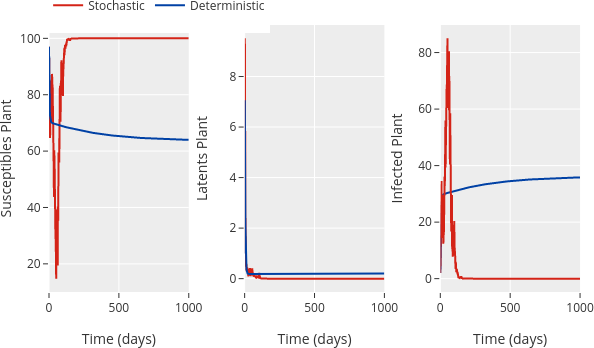
\includegraphics[scale=0.45, keepaspectratio]{%
	Figures/ExtinctionNoise.png}
	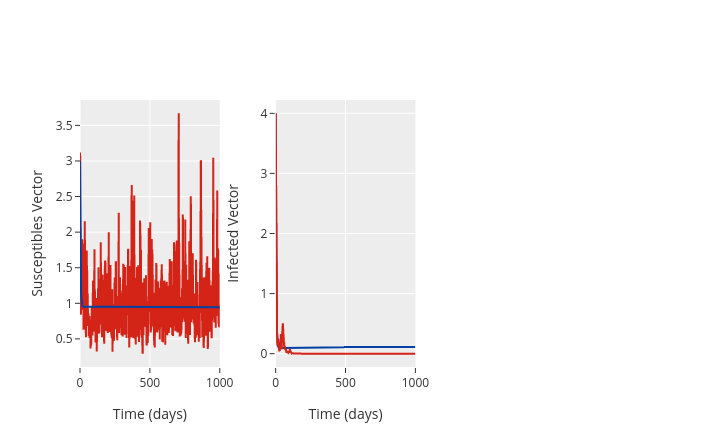
\includegraphics[scale=0.45, keepaspectratio]{%
	Figures/ExtinctionNoiseVector.png}
	\end{center}
	\caption{%
		\href{https://plotly.com/~AdrianSalcedo/2/}{%
		https://plotly.com/~AdrianSalcedo/2/}}
	\label{fig:ExtinctionByNoise}
\end{figure}
\begin{figure}[ht]
	\centering
	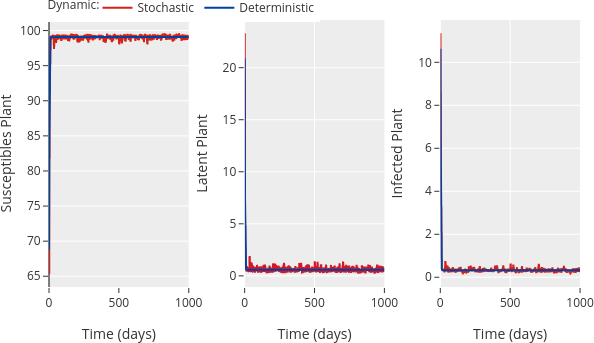
\includegraphics[scale=0.45, keepaspectratio]{%
	Figures/Rs0LessThanOne.png}
	
	\caption{Here we present the $\mathcal{R}^s_0<1$ only plant population}
	\label{fig:Rs0SmallerThanOne}
\end{figure}
\info{Include infected vector dynamics}
\begin{figure}[ht]
	\centering
	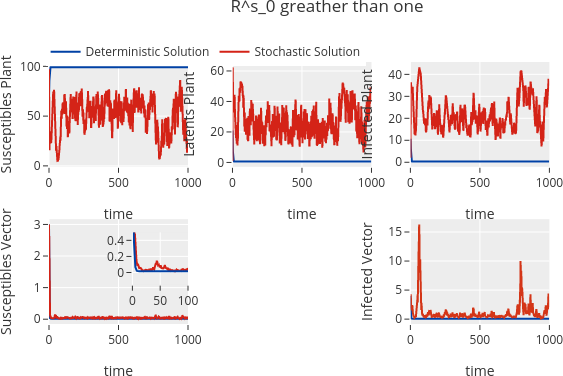
\includegraphics[scale=0.5, keepaspectratio]{%
	Figures/R0_more/R^s_0greather_than_one.png}
	\caption{Caption two}
	\label{fig:Rs0GreatherThanOne}
\end{figure}

\info{Make GitHub repository and bib reference}
\change{Enumerate plot panels}
	\section{Conclusion}
	    \todo{Write a proposal}
		\label{sec:conclusion}
	    \paragraph{Findings}
1. We established by algebraic manipulations basic reproductive number
$\mathcal{R}^s_0$ for \autoref{sys::StochasticSystem}. We observe that
$\mathcal{R}^s_0$ is a threshold parameter as the deterministic case.
\paragraph{Judgment}
2. With this threshold parameter, we can establish preventive measures to reduce
the spread of the disease in the crop. With this, we obtain a greater production.
In the definition of $\mathcal{R}^s_0$ it is observed that the most significant
measures are replanting and fumigation. If we take into account increasing said
prevention measures against the disease we will obtain a more productive crop.
\paragraph{Limitations}
One of the complications found is the fact of getting the most out of replanting
for latent and infected plants. 
\paragraph{Perspectives}
4. suggestions for improvements (perhaps in relation to the limitations)
To improve this, I would like to investigate some technique to obtain the
stochastic basic reproductive number in terms of each replanting rate for plants.

5. recommendations for future work (either for the author, and/or the community)
For a future work, I would like to apply the theory of stochastic
control to \autoref{sys::StochasticSystem} be able to give control
measures over the disease, based on which strategy is most beneficial
and why to carry it out.


	\section{Here the fucking todo list. Task due to Junary 12 2021}
	\listoftodos
	\appendix
	\section{Background 1}
	Given a function 
$
	V\in C^{2,1}(\R^n\times\R_{+};\R)
$, 
define an operator 
$
	\mathcal{L}[V]:\R ^ n \times \R_{+}\to\R
$ by
\begin{equation}\label{eqn::DifussionOperator}
	\mathcal{L}[V(x,t)] = 
		V_t(x,t) + 
		V_x(x,t) f(x,t) + 
		\frac{1}{2} 
		\trace(g^T(x,t)V_{xx}(x,t)g(x,t))
\end{equation}
%
which is called the diffusion operator of the It\^{o} process associated with 
the $C^{2,1}$ function $V$. With this diffusion operator, the It\^{o} formula 
can be written as
\begin{equation}\label{eqn::Itoformula}
	dV(x(t),t) = 
		\mathcal{L}
			V(x(t),t)dt + 
			V_x(x(t), t) 
			g(x(t),t) dB(t) \qquad a.s.
\end{equation}
\begin{theorem}
Here Khaminskii theorem
\end{theorem}
	\label{app::A}
	\section{Background 2}
	\begin{theorem}\label{thm::YoungInequality}
    If $a$ and $b$ are non negative real numbers and $p$ and $q$ are real numbers greater than $1$ such that 
    $\frac{1}{p} + \frac{1}{q} = 1$, then
    \begin{equation*}
        ab\leq \frac{a^p}{p} + \frac{b^q}{q}.
    \end{equation*}
\end{theorem}
The limit inferior of a sequence $\{x_n\}$ is defined by

\begin{equation}\label{eqn::limitInf}
    \liminf_{n\to \infty}x_n :=\lim_{n \to \infty}\left(\inf_{m\geq n}x_m\right).
\end{equation}

Similarly, the limit superior of $\{x_n\}$ is defined by 

\begin{equation}\label{eqn::limitSup}
    \limsup_{n\to \infty}x_n :=\lim_{n \to \infty}\left(\sup_{m\geq n}x_m\right).
\end{equation}

The relationship of limit inferior and limit superior for sequences of real numbers is as follows:

\begin{equation}\label{eqn::propertybetween}
   \limsup_{n \to \infty} (-x_n) = -\liminf_{n \to \infty} x_n.
\end{equation}
	\label{app::B}
	\bibliography{Ref_Book,Ref_Article}{}
    \bibliographystyle{spmpsci}
	\info{add a tex source with the appendix files}
\end{document}
